% Hvordan implementerte jeg dette i praksis?


% Data aquisition 
% DATA transfer
% Offline processing
% feature extraction

%\section{System Architecture}
%    \subsection{Block Diagram} 
%    \subsection{Signal Flow}

\section{3D design}
\subsection{PAN and Tilt mechanism}

The camera platform is a modified version of this pan tilt camera setup (\cite{isaac879_2020_pantilt}) with all files being created using fusion 360. At first a Prusa Slicer mini with 0.4mm nozzle diameter was used for the intial prints. With the later prints being done using a Bambu lab P2S  3D printer with a 0.4mm nozzle diameter. 

\begin{figure}[H]
    \centering
    \begin{subfigure}{0.45\linewidth}
        \centering
        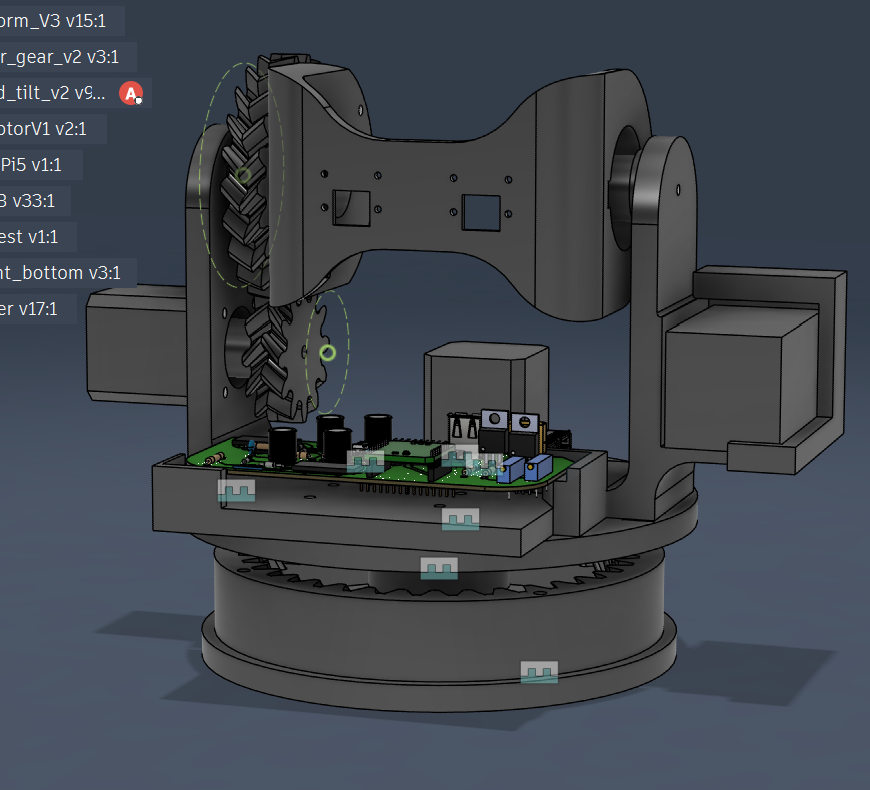
\includegraphics[width=\linewidth]{Figures/Andreas/3D Design/Full_assembly_V1.png}
        \caption{3D CAD design}
        \label{fig:full_assembli}
    \end{subfigure}
    \hfill
    \begin{subfigure}{0.45\linewidth}
        \centering
        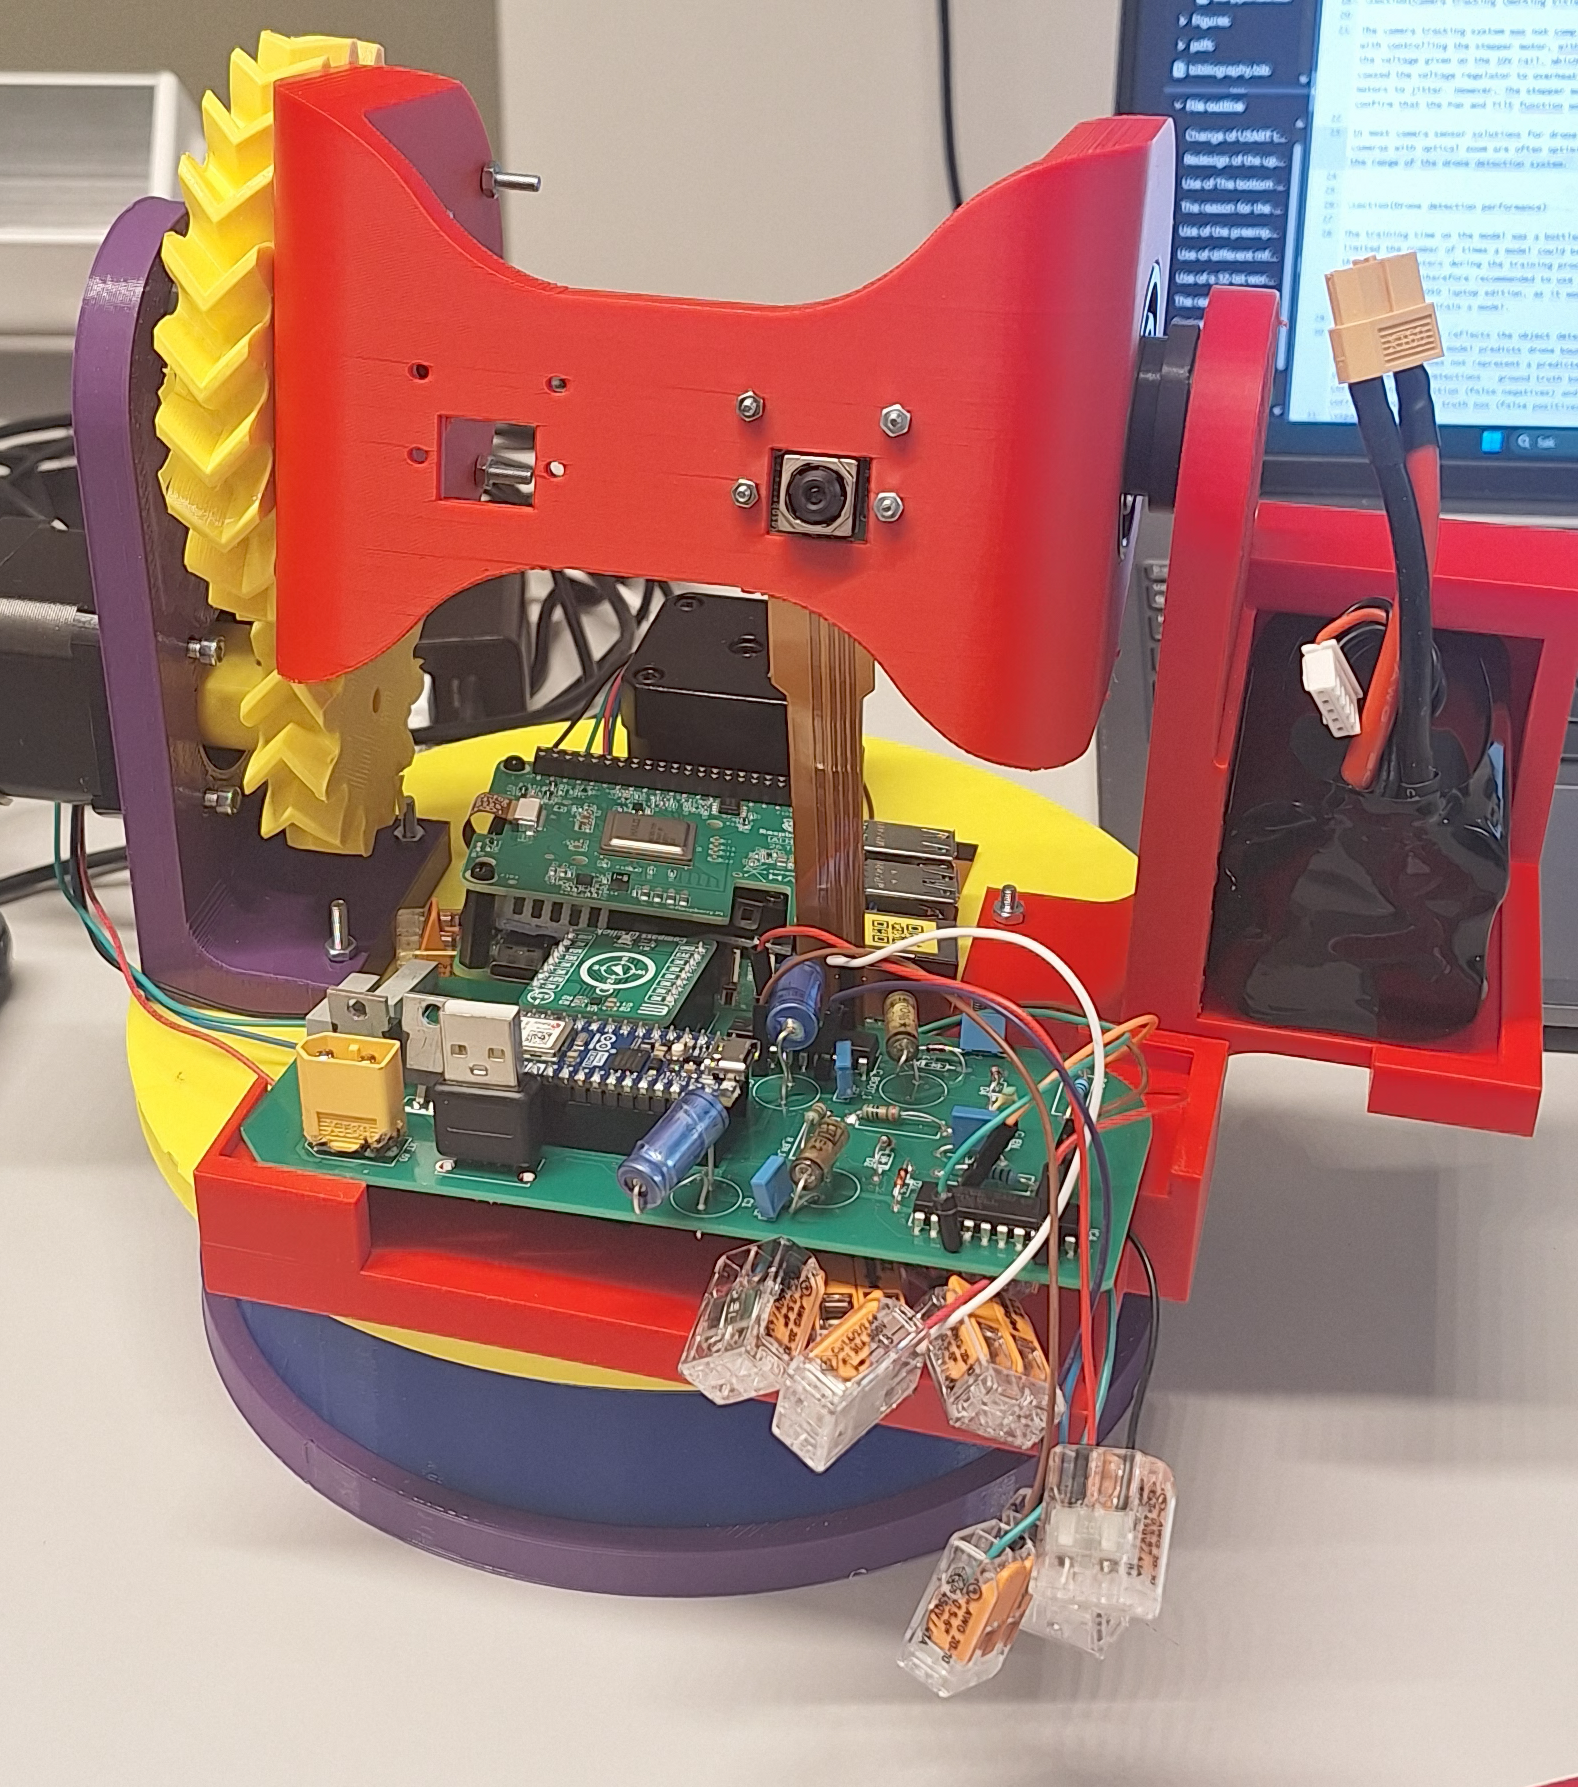
\includegraphics[width=\linewidth]{Figures/Andreas/3D Design/Full_print.png}
        \caption{Final printed version}
        \label{fig:full_print}
    \end{subfigure}
    \caption[3D design camera platform]{3D design camera platform}
    \label{fig:full_assembly_pair}
\end{figure}

The horizontal camera movement is controlled by a stepper motor connected to an 8 teeth gear which 
rotates around a 37 teeth track, giving it a full 360° rotation (fig: \ref{fig:pan_mechanism}). 
The gear ratio is $\frac{37}{8} = 4.625$, meaning the motor must complete 4.625 full rotations to 
rotate the platform 360°. Since each step of the stepper motor is 1.8°, one full motor rotation 
requires $\frac{360°}{1.8°} = 200$ steps, resulting in a total of $200 \times 4.625 = 925$ steps 
per full platform rotation, giving an angular resolution of $\frac{360°}{925} \approx 0.39°$ per step.

\begin{figure}[H]
    \centering
    \begin{subfigure}{0.45\linewidth}
        \centering
        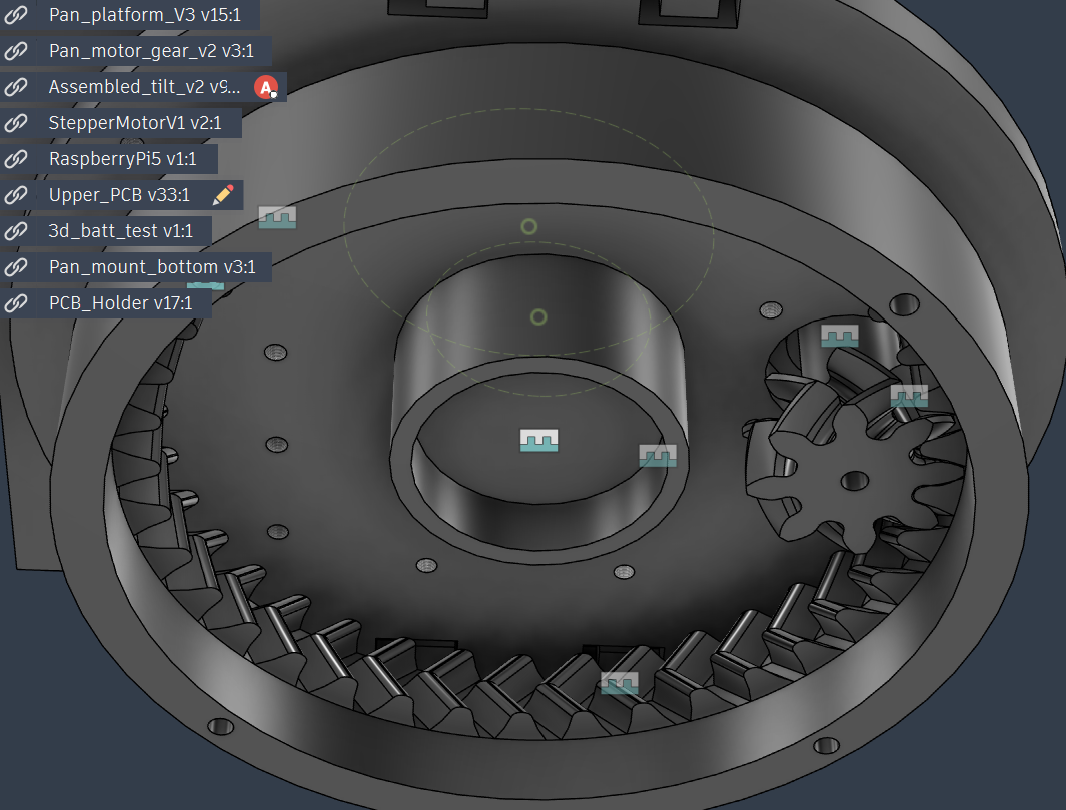
\includegraphics[width=\linewidth]{Figures/Andreas/3D Design/Pan_mechanism_V1.png}
        \caption{Screenshot from Fusion 360 of the pan mechanism.}
        \label{fig:pan_mechanism}
    \end{subfigure}
    \hfill
    \begin{subfigure}{0.35\linewidth}
        \centering
        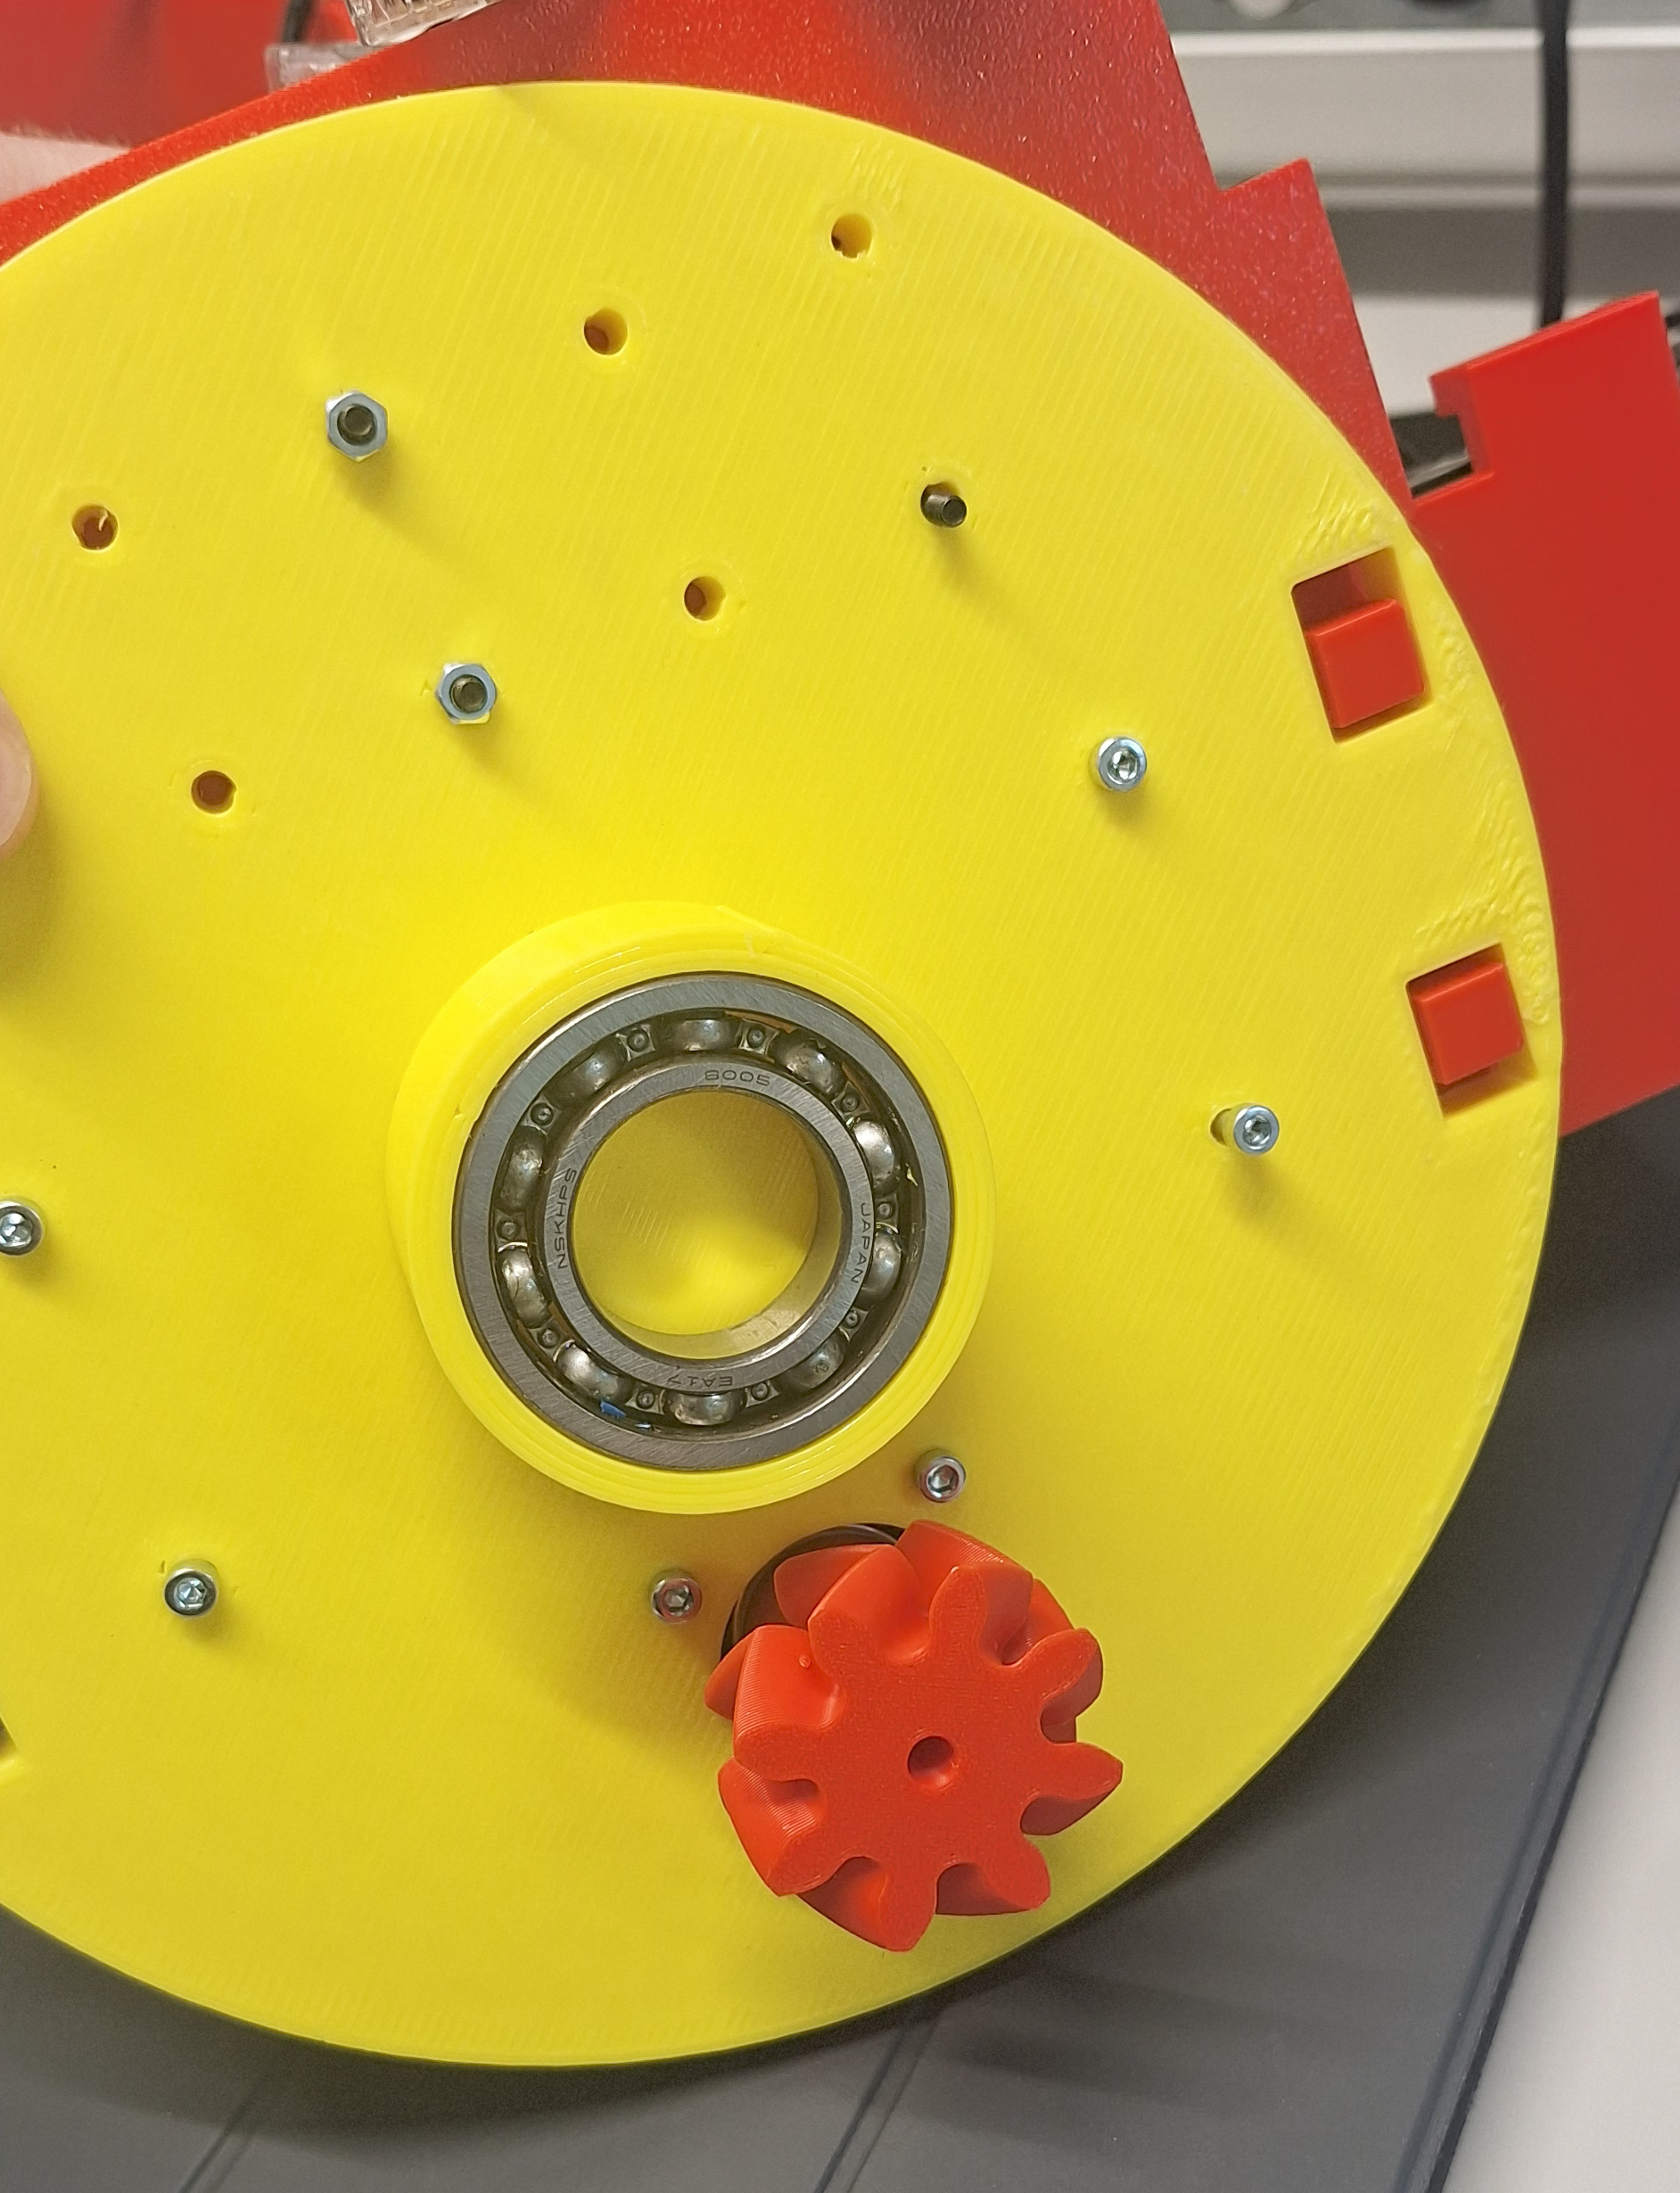
\includegraphics[width=\linewidth]{Figures/Andreas/3D Design/Bottom_ball_bearing.png}
        \caption{Image of the underside of the pan mechanism}
        \label{fig:bottom_ball_bearing}
    \end{subfigure}
    \caption[Pan mechanism]{Pan mechanism}
    \label{fig:pan_pair}
\end{figure}

The vertical camera movement is controlled by a stepper motor connected to a 12 teeth herringbone 
gear turning a larger 24 teeth herringbone gear (fig: \ref{fig:tilt_mechanism}). The gear ratio is 
$\frac{24}{12} = 2$, meaning the motor must complete 2 full rotations to rotate the camera 360°. 
With each step being 1.8°, one full motor rotation requires 200 steps, resulting in a total of 
$200 \times 2 = 400$ steps per full camera rotation, giving an angular resolution of 
$\frac{360°}{400} = 0.9°$ per step.

\begin{figure}[H]
    \centering
    \begin{subfigure}{0.45\linewidth}
        \centering
        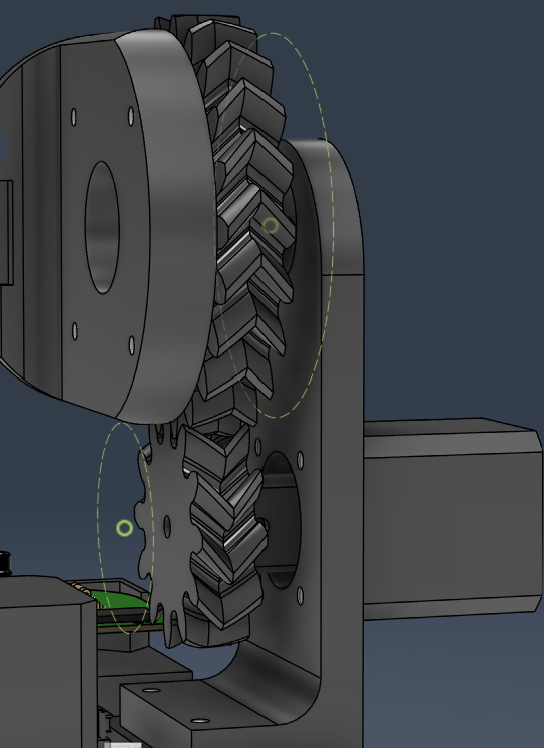
\includegraphics[width=\linewidth]{Figures/Andreas/3D Design/Tilt_mechanism_V1.png}
        \caption{Screenshot from Fusion 360 showing the tilt mechanism.}
        \label{fig:tilt_mechanism}
    \end{subfigure}
    \hfill
    \begin{subfigure}{0.45\linewidth}
        \centering
        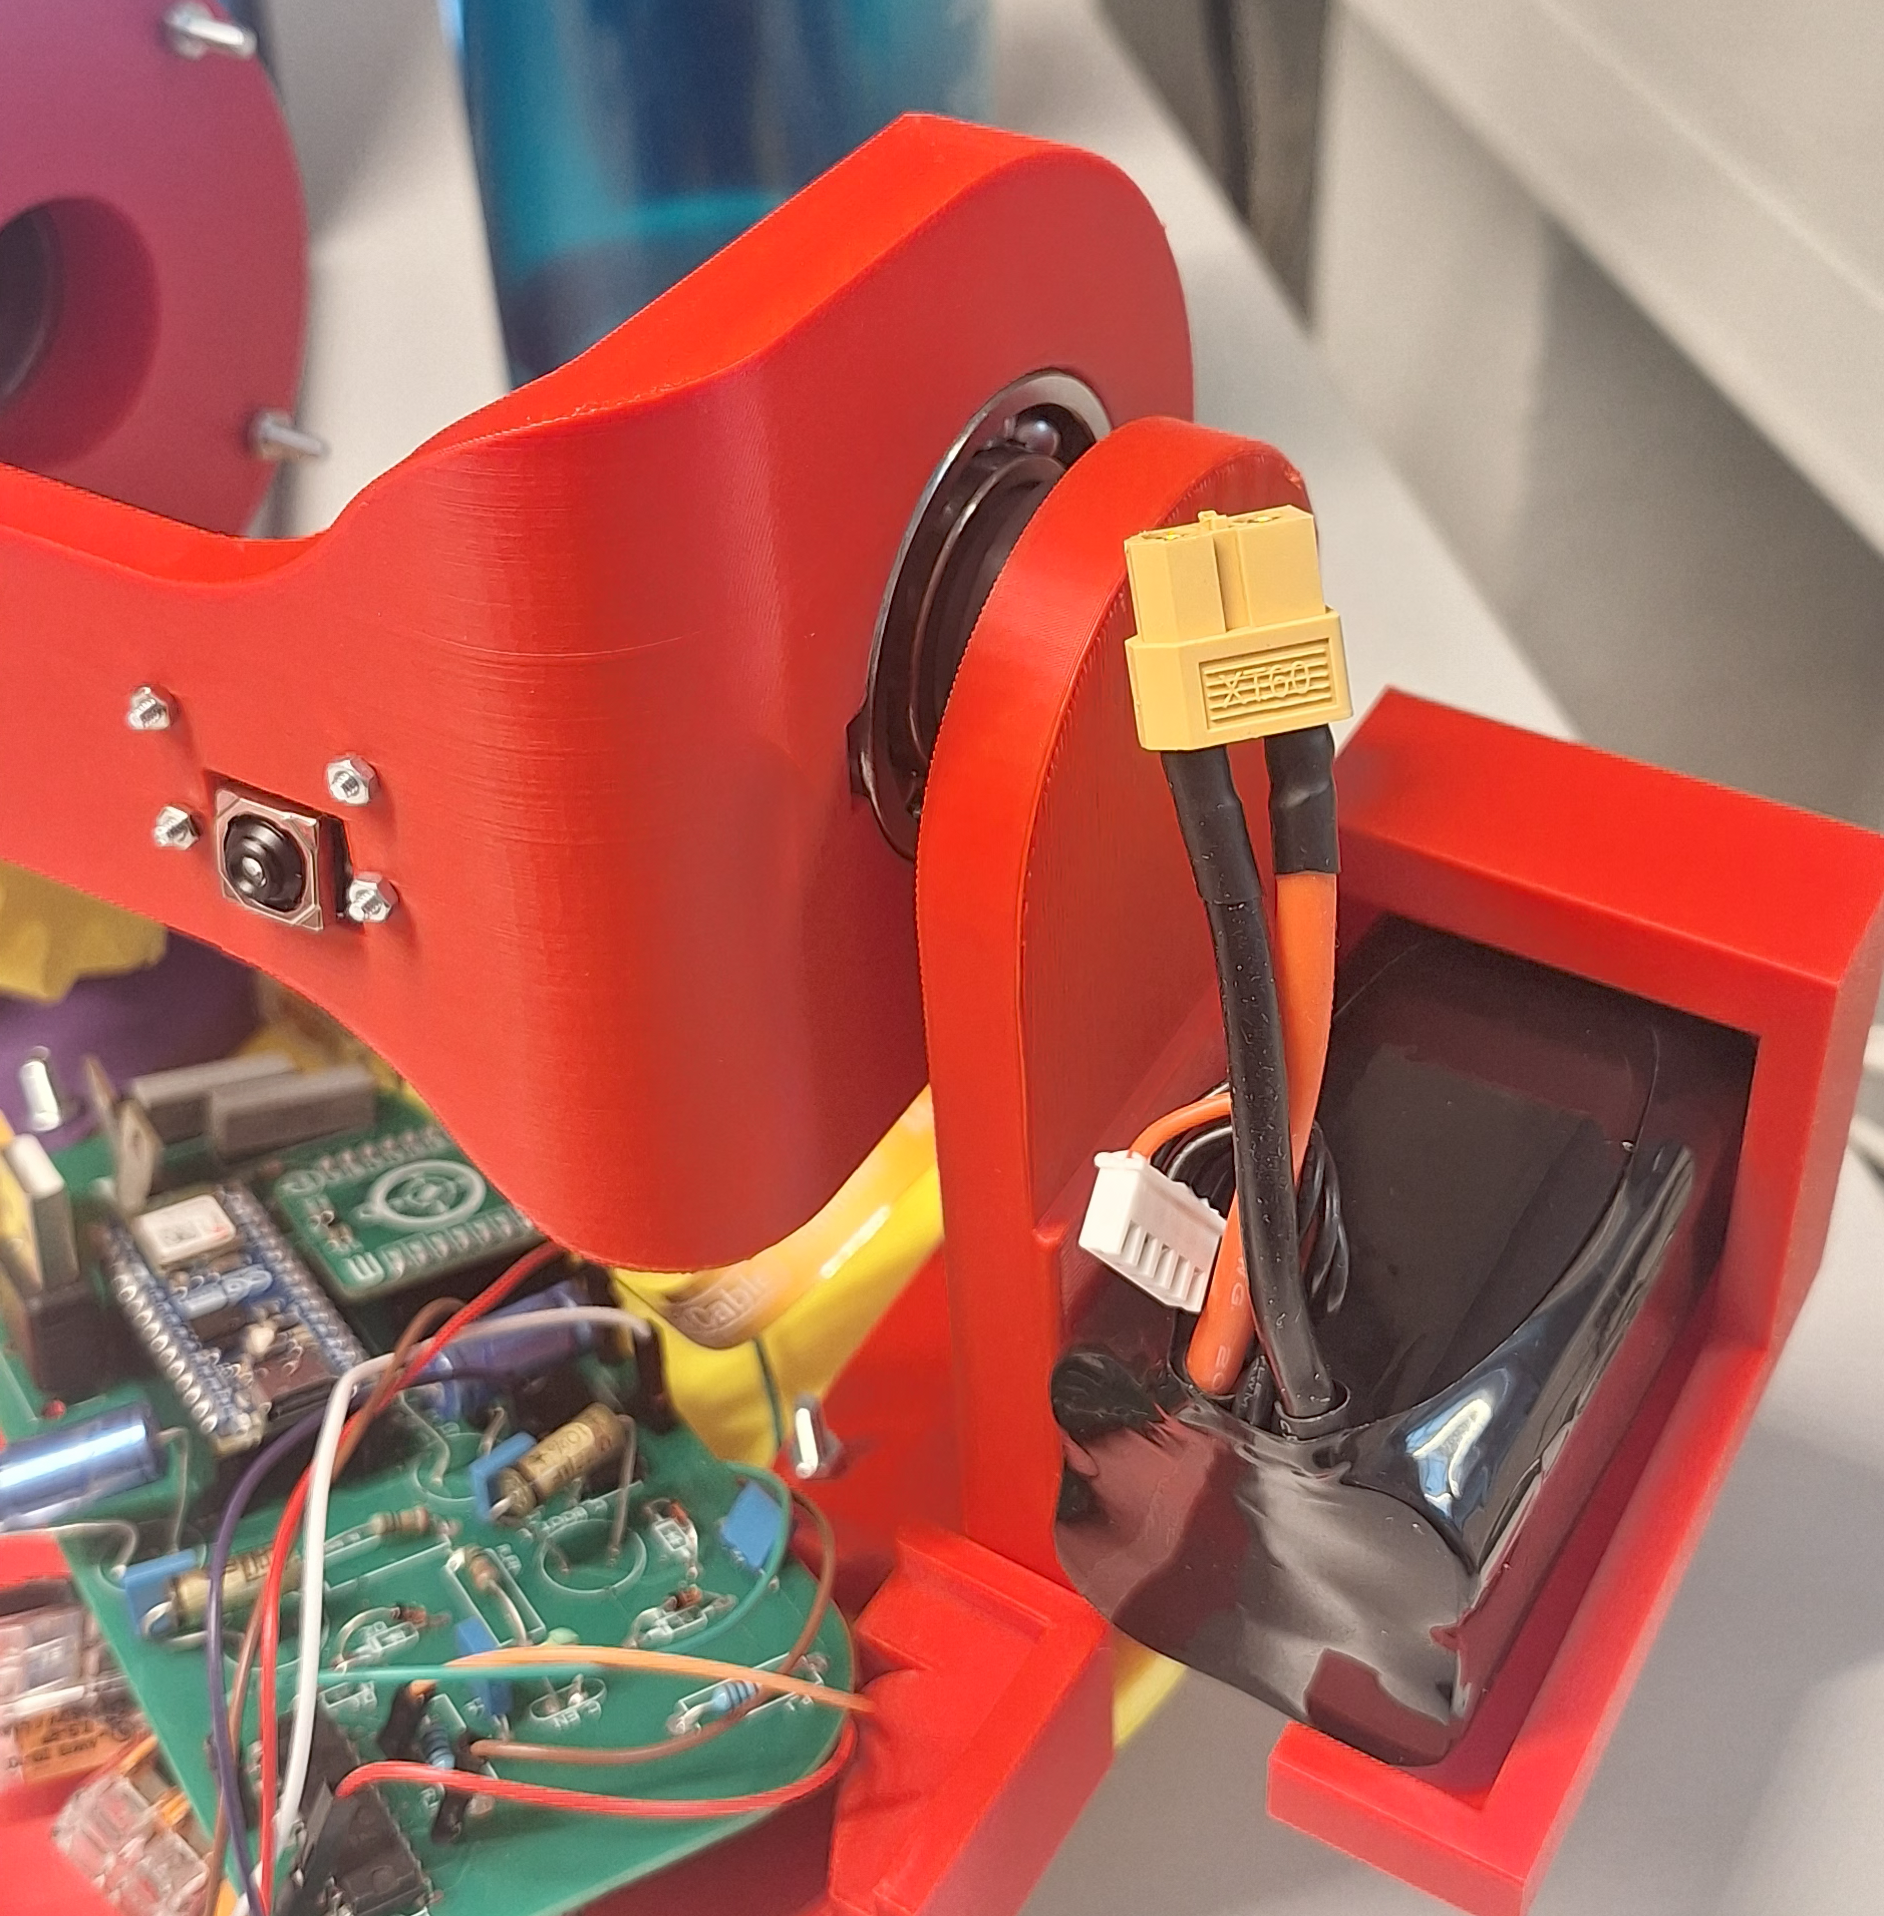
\includegraphics[width=\linewidth]{Figures/Andreas/3D Design/Side_ball_bearing.png}
        \caption{Ball bearing on the opposite side.}
        \label{fig:side_ball_bearing}
    \end{subfigure}
    \caption[Tilt mechanism]{Tilt mechanism}
    \label{fig:tilt_pair}
\end{figure}


\section{Hardware costs}

\begin{table}[h]
\centering
\caption{Equipment List with Prices for the system}
\label{tab:equipment}
\begin{tabular}{|l|l|r|}
\hline
\textbf{Component} & \textbf{Description} & \textbf{Price (NOK)} \\
\hline
Battery & Bronto 4S 5000mAh 21700 Li-Ion XT60 & 829 \\
\hline
Raspberry Pi 5 & 8 GB RAM & 2\,099 \\
\hline
Raspberry Pi AI HAT+ & AI accelerator add-on, 26 TOPS & 1\,499 \\
\hline
Raspberry Pi Camera Module & Camera for image capture & 509 \\
\hline
Stepper Motor $\times$2 & (2 units) & 962 \\
\hline
Compass & MikroElektronika Compass 6 Click, & 419 \\
\hline
Arduino Nano ESP32 & Microcontroller & 193 \\
\hline
Ball Bearing $\times$3 & ID 25\,mm, OD 47\,mm (3 units) & 240 \\
\hline 
STM32F413 & MCU for signal processing & 372 \\ 
\hline
PCB & Upper and bottom (has to buy 5x) & 700 \\ 
\hline
STEVAL-MIC002V1 & Microphone array (has 4 microphones) & 400 \\
\hline
L6205N & Motor controller (2x) & 200\\
\hline
Div electronics & resistors, voltage regulators etc. & 300 \\
\hline
\hline
\textbf{Camera Only total} & & \textbf{4\,517} \\
\hline
\textbf{Total} & & \textbf{8\,503} \\
\hline
\end{tabular}
\end{table}

\section{Acoustic Signal Acquisition and Analysis}
This section provides the explenation on how the acoustic signal was gathered and analysed to extract its spectrum and estimate the signals source of origin.


\subsection{Hardware Implementation for sound acquisition}
    \subsubsection{Microphone array and The expantion board} 
    The project uses an \href{https://www.st.com/resource/en/data_brief/steval-mic002v1.pdf}{\textbf{STEVAL-MIC002V1}} microphone array, which consists of four \href{https://www.st.com/resource/en/datasheet/mp34dt06j.pdf}{\textbf{MP34DT06J}} digital MEMS microhpones. The microphones are positioned as shown in Figure~\ref{fig:mics_on_the_tower}. Each microphone is placed 10 cm from the center of the platform along either the \textbf{X}-axis or \textbf{Y}-axis. All microphones are positioned in the same horizonatal plane, so the \textbf{Z}-coordinate, is set to zero for all micropohone positions. The position vector initialized in the \textbf{main.py} that describes the microphones position in relation to the platforms center, can be seen in Figure~\ref{fig:p_vector}. The microphones (beside the data pins) are connected to the \textbf{M1/2\_EXT} pins at the \href{https://www.st.com/en/evaluation-tools/x-nucleo-cca02m2.html}{\textbf{CCA02M2}} extantion board as seen in Figure~\ref{fig:CCA02M2_connection}. The CCA02M2 is used to supply the microphones with the clock signal and the 3.3V supply from the MCU. The board also allows to send the data signal from two microphones on the same line, by setting L/R pin high or low. That functionality was not used in the final stage of the project, as the data signal from the microphones is send directly to each microphone's own channel at the MCU, which directs the signal further to the connected DF. The extantion board is also used to send the PCM values from the MCU to the connected raspberry Pi or PC, through a micro usb which needs its own 5V supply, that is also provided by the connected MCU.

    \begin{figure}[h]
        \centering
        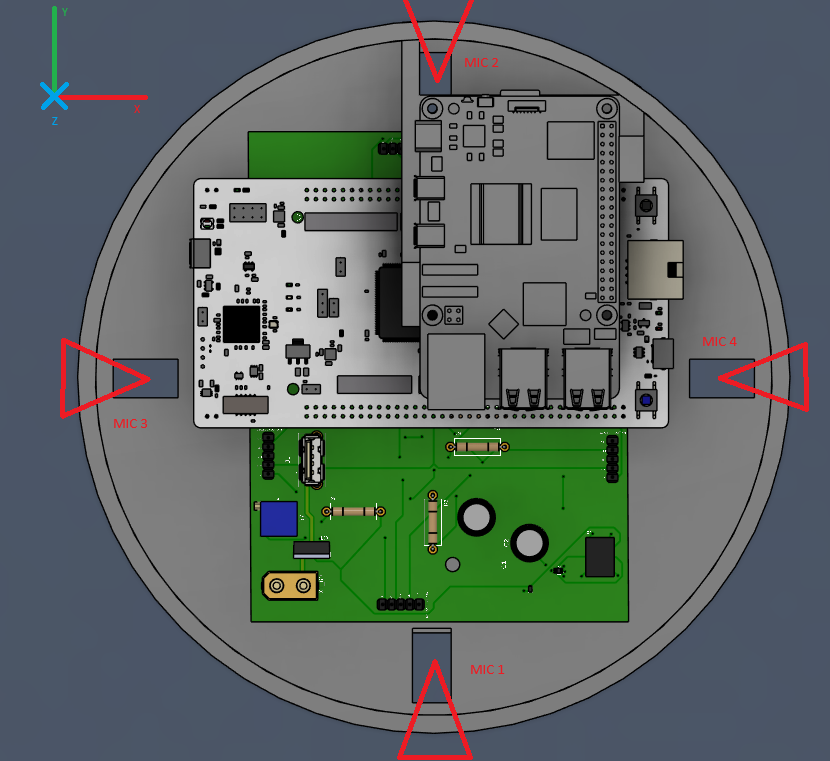
\includegraphics[width=0.75\linewidth]{Figures/mics.png}
        \caption[  The microphones placement]{The placement of the microhpones on the bottom part of the tower.}
        \label{fig:mics_on_the_tower}
    \end{figure}

    \begin{figure}[h]
        \centering
        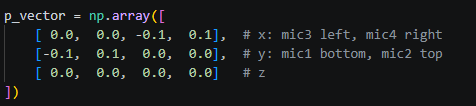
\includegraphics[width=0.5\linewidth]{Figures/p_vector.png}
        \caption[  P-vector]{P vector that represents the position of each microphone in relation to the platform center.}
        \label{fig:p_vector}
    \end{figure}

    \begin{figure}[h]
        \centering
        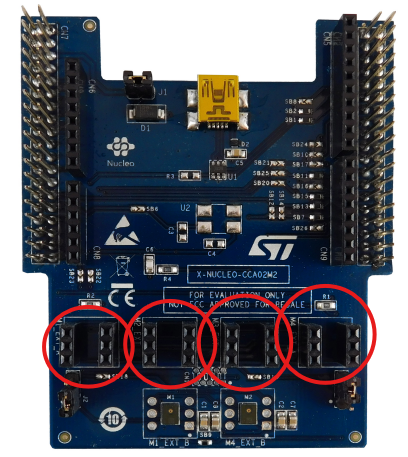
\includegraphics[width=0.5\linewidth]{Figures/cca02m2.png}
        \caption[  CCA02M2]{The CCA02M2 used in the project marked with outputs used for microphone connection. Source: \cite{x_nucleo_cca02m2_2019}.}
        \label{fig:CCA02M2_connection}
    \end{figure}

\newpage
    \subsubsection{STM32 configuration}
    The \href{https://www.st.com/en/microcontrollers-microprocessors/stm32f413zh.html#st_description_sec-nav-tab}{\textbf{F413ZH}}, is the MCU of STM32 model used in the final version of the project, and the reasoning for why this particular model was chosen, can be accessed in Section~\ref{sec:stm32_models_reasoning}.
    The STM32 was configured in CubeMX to use the I/O seen in Figure~\ref{fig:pinout_cubemx} and was phisically connected as in the Figure~\ref{}. The MCU supplies the extanstion board with the 3.3V and 5V signal, and sends the PCM data through it. The MCU, uses the peripherals seen in the Figure~\ref{fig:system_view_peripherals}, and some of them will be explained in the following sections.

    \begin{figure}[h]
        \centering
        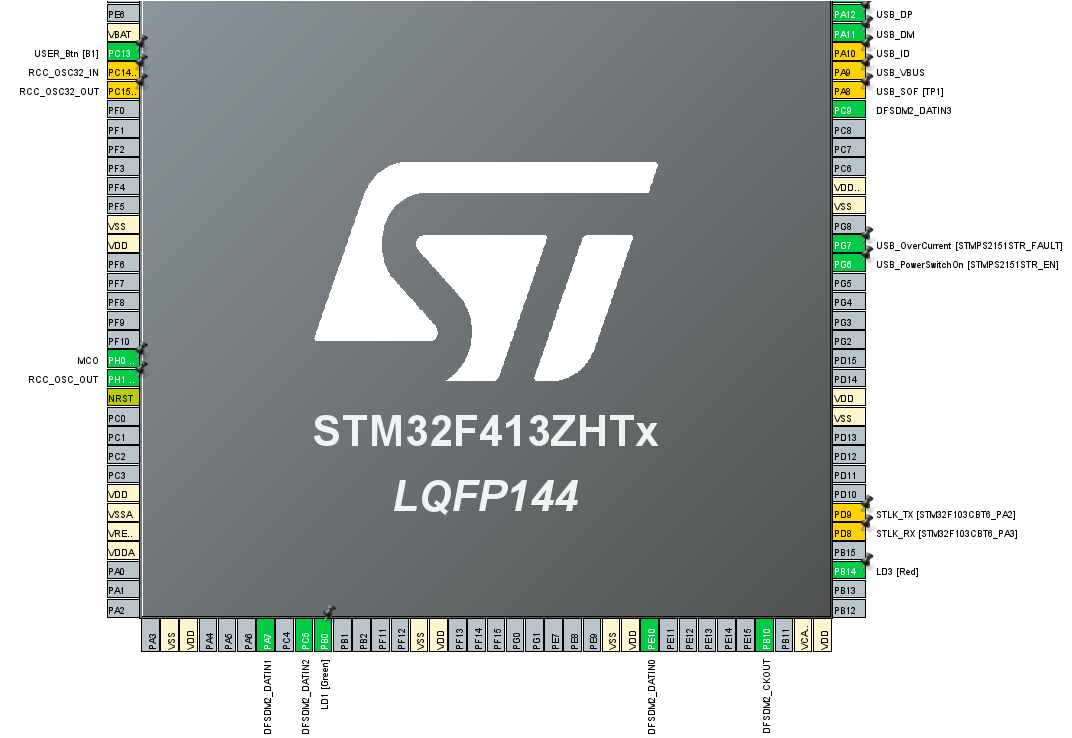
\includegraphics[width=0.75\linewidth]{Figures/pinout_cubemx.png}
        \caption[  STM32 pinout]{The pinout view of the STM32 F413ZH used in the project.}
        \label{fig:pinout_cubemx}
    \end{figure}


    \begin{figure}[h]
        \centering
        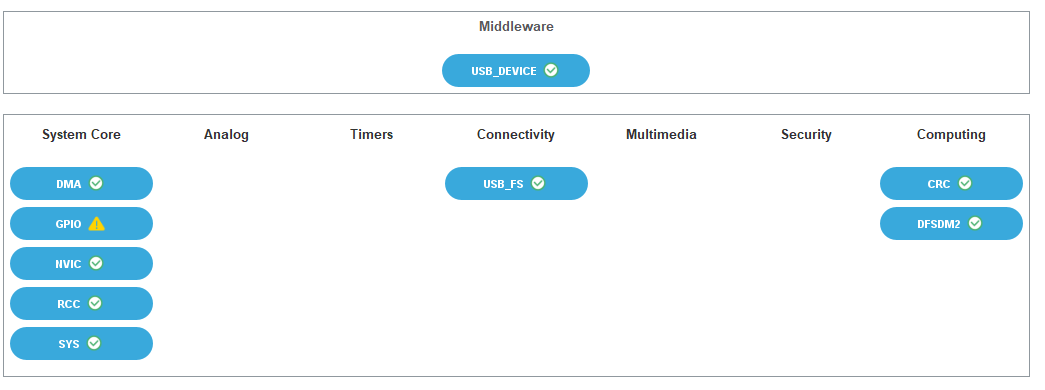
\includegraphics[width=0.5\linewidth]{Figures/system_view.png}
        \caption[  MCU peripherals]{System view of the MCUs peripherals}
        \label{fig:system_view_peripherals}
    \end{figure}
    \newpage
    
    \subsubsection{DFSDM configuration}
    The DFSDM was configured to be able to gather the acoustic signals from four microphones, hence the use of four separate channels as seen in Figure~\ref{fig:DFSDM2_modes}. But for the microphones to be able to send any data signal, they first have to be supplied by the clock signal, that they could use to adjust the data frequency to. The clock signal can be generated by the internal to the MCU clock as in Figure~\ref{fig:clock_dfsdm2}, which was set to 16Mhz. The clock signal is later reduced to around 2 Mhz and relied to the microphones by the \textbf{PB10} pin. 
    
    \begin{figure}[h]
        \centering
        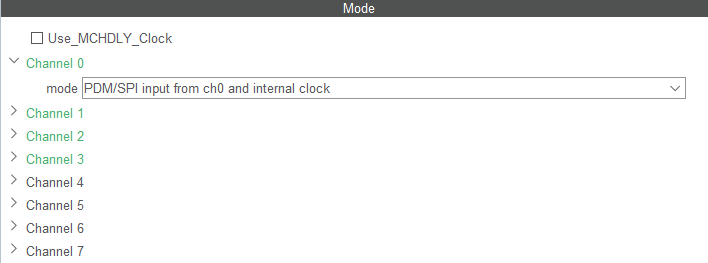
\includegraphics[width=0.5\linewidth]{Figures/modes_dfsdm.png}
        \caption[  DFSDM2 modes]{Modes in which the DFSM2 is configured}
        \label{fig:DFSDM2_modes}
    \end{figure}

    \begin{figure}[h]
        \centering
        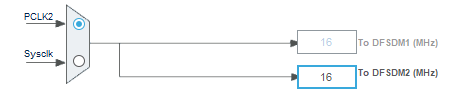
\includegraphics[width=0.5\linewidth]{Figures/DFSDM2_clock_config.png}
        \caption[  Clock for DFSDM2]{The clock frequency of the DFSDM2}
        \label{fig:clock_dfsdm2}
    \end{figure}
    \newpage

    

    If the signals from two microphones would be placed on the same line, type of the signal would have to be specified to either \textbf{SPI with falling edge} or \textbf{SPI with rising edge} as in Figure~\ref{fig:config_firstchannel} so that the signals could be properly deinterleaved. The channels watchdog can also be configured to monitor the signals behaviour, hovewer that functionality was not implememented in the final design.

    \begin{figure}[h]
        \centering
        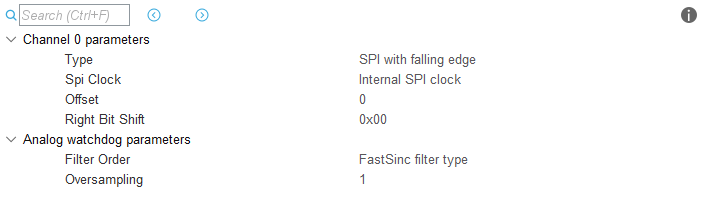
\includegraphics[width=0.5\linewidth]{Figures/channel0_config.png}
        \caption[  First DFSDM channel config]{Configuration of the first channel of the DFSDM.}
        \label{fig:config_firstchannel}
    \end{figure}
    \newpage

    Each filter was configured as in Figure~\ref{fig:config_filter_dfsdm}, where the main functions used are: the filter parameters of \textbf{Sinc Order} which was chosen to be of the 3th order, and the oversampling ratio \textbf{FOSR} of 32.  

    \begin{figure}[h]
        \centering
        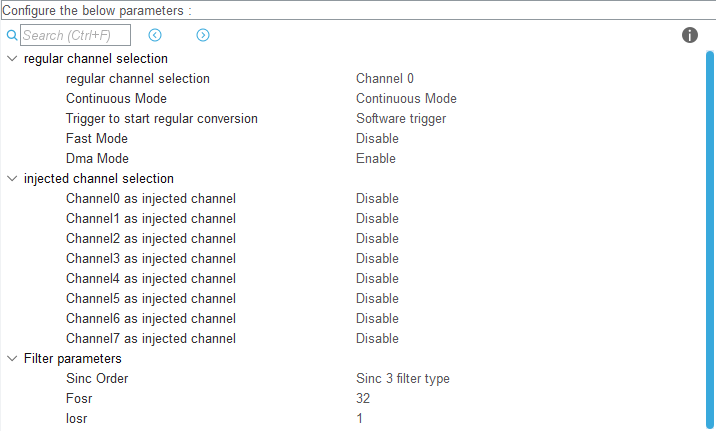
\includegraphics[width=0.5\linewidth]{Figures/filter_config_dfsdm.png}
        \caption[  Each filter config for DFSDM]{Configuration of each filter applied in DFSDM.}
        \label{fig:config_filter_dfsdm}
    \end{figure}

    The reason for the use of thesse values is that the third order sinc function, seamed to provide a reasonable balance between the sidelobe reduction and noise attenuation against the attenuation of the desired frequencies as seen in Figure~\ref{fig:mag_response_sinc}. The FOSR was selected to reduce the PDM bitstream to a lower PCM output rate while still maintaining a sampling frequnecy high enough to represent the relevant acoustic signal.  \\
 
    In the \textbf{main.c} in the STM32 project, the filter and channel handlers were declared as in Code~\ref{lst:dfsdm_filter_objects_declarations}, and later configured to operate togheter in the continous mode as in Code~\ref{lst:dfsdm_filter_config}, to insure that each channel is connected to the correct filter and that they sample and filter the microphone data correctly.\\

     \begin{lstlisting}[style=cstyle, caption={Declarations of the filter and channel objects}, label={lst:dfsdm_filter_objects_declarations}]
    DFSDM_Filter_HandleTypeDef hdfsdm2_filter0;
    DFSDM_Filter_HandleTypeDef hdfsdm2_filter1;
    DFSDM_Filter_HandleTypeDef hdfsdm2_filter2;
    DFSDM_Filter_HandleTypeDef hdfsdm2_filter3;
    DFSDM_Channel_HandleTypeDef hdfsdm2_channel0;
    DFSDM_Channel_HandleTypeDef hdfsdm2_channel1;
    DFSDM_Channel_HandleTypeDef hdfsdm2_channel2;
    DFSDM_Channel_HandleTypeDef hdfsdm2_channel3;
    \end{lstlisting}
    
    \begin{lstlisting}[style=cstyle, caption={Linking a DFSDM regular channel to a filter in continuous conversion mode}, label={lst:dfsdm_filter_config}]

if (HAL_DFSDM_FilterConfigRegChannel(&hdfsdm2_filter0,
                                       DFSDM_CHANNEL_0,
                                       DFSDM_CONTINUOUS_CONV_ON) != HAL_OK)
{
    Error_Handler();
}
    \end{lstlisting}
   \newpage
    \subsubsection{DMA buffering}
    The DMA was configured as in Figure~\ref{fig:dma_config}, to transfer the samples produced by the DFSDM peripheral to the internal memory of the MCU. Circular mode was used so that the DMA buffer could be reused continously during audio acquisition. When the end of the buffer is reached, the DMA controller starts writing the data from the begining of the buffer again, allowing for continous sampling. The Data samples were chosen to be stored as the 32-bit words in the DMA buffer, before the further processing and conversion. 
    
    \begin{figure}[h]
        \centering
        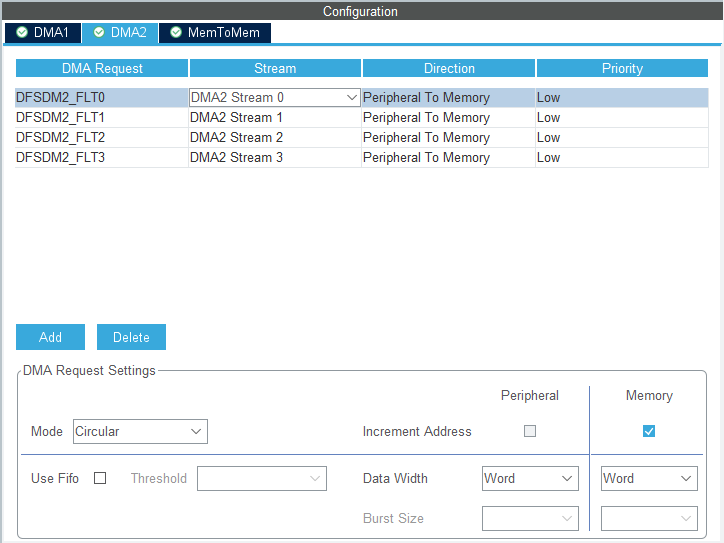
\includegraphics[width=0.5\linewidth]{Figures/dma_config.png}
        \caption[  DMA config]{Configuration of the DMA streams.}
        \label{fig:dma_config}
    \end{figure}

    The pcm buffers are declared as in the following Code~\ref{lst:PCM_buffer_declarations}. Each DFSDM filter has a dedicated DMA buffer declared as \textbf{int32\_t}, since the DFSDM peripheral outputs 32-bit samples. The buffer length is defined as twice the number of PCM samples used per half-buffer. This creates a double-buffer structrue, where one half of the buffer can be processed and send while the DMA is filling the other half. That is possible by setting the flags high for when the buffer is half full and completly full as shawn in Code~\ref{lst:callbacks_half_full}.
    The DMA handlers are declared as shawn in Code~\ref{lst:DMA_filter_obj}. These handlers are then used when starting the DFSDM regulator conversion with DMA as shawn in Code~\ref{lst:dfsdm_filter_to_pcm_buffer}. This connects each DFSDM filter output to its corresponding DMA buffer so that the converted samples are written to the memory. 
    
    \begin{lstlisting}[style=cstyle, caption={PCM buffers declaration}, label={lst:PCM_buffer_declarations}]
    
    #define PCM_SAMPLES_PER_HALF  16
    #define DFSDM_DMA_SAMPLES     (PCM_SAMPLES_PER_HALF * 2)
    
    static int32_t pcm0_dma[DFSDM_DMA_SAMPLES];
    static int32_t pcm1_dma[DFSDM_DMA_SAMPLES];
    static int32_t pcm2_dma[DFSDM_DMA_SAMPLES];
    static int32_t pcm3_dma[DFSDM_DMA_SAMPLES];
    \end{lstlisting}

    \begin{lstlisting}[style=cstyle, caption={Declaration of the DMA objects}, label={lst:DMA_filter_obj}]
    DMA_HandleTypeDef hdma_dfsdm2_flt0;
    DMA_HandleTypeDef hdma_dfsdm2_flt1;
    DMA_HandleTypeDef hdma_dfsdm2_flt2;
    DMA_HandleTypeDef hdma_dfsdm2_flt3;
    \end{lstlisting}
\newpage    
    \begin{lstlisting}[style=cstyle, caption={Connecting a DFSDM filter output to its dedicated DMA buffer}, label={lst:dfsdm_filter_to_pcm_buffer}]
     if (HAL_DFSDM_FilterRegularStart_DMA(&hdfsdm2_filter0, pcm0_dma, DFSDM_DMA_SAMPLES) != HAL_OK)
  {
      Error_Handler();
  }
  \end{lstlisting}

  \begin{lstlisting}[style=cstyle, caption={DMA half-complete and complete callbacks for DFSDM filter buffers. Generated by \cite{chatgpt2026}, although somewhat modified during the debuging process by adding the counter to each filter.}, label={lst:callbacks_half_full}]

    void HAL_DFSDM_FilterRegConvHalfCpltCallback(DFSDM_Filter_HandleTypeDef *hdfsdm_filter)
{
    if (hdfsdm_filter->Instance == DFSDM2_Filter0) { flt0_half_ready = 1; cb_half0++; }
    if (hdfsdm_filter->Instance == DFSDM2_Filter1) { flt1_half_ready = 1; cb_half1++; }
    if (hdfsdm_filter->Instance == DFSDM2_Filter2) { flt2_half_ready = 1; cb_half2++; }
    if (hdfsdm_filter->Instance == DFSDM2_Filter3) { flt3_half_ready = 1; cb_half3++; }
}

void HAL_DFSDM_FilterRegConvCpltCallback(DFSDM_Filter_HandleTypeDef *hdfsdm_filter)
{
    if (hdfsdm_filter->Instance == DFSDM2_Filter0) { flt0_full_ready = 1; cb_full0++; }
    if (hdfsdm_filter->Instance == DFSDM2_Filter1) { flt1_full_ready = 1; cb_full1++; }
    if (hdfsdm_filter->Instance == DFSDM2_Filter2) { flt2_full_ready = 1; cb_full2++; }
    if (hdfsdm_filter->Instance == DFSDM2_Filter3) { flt3_full_ready = 1; cb_full3++; }
}

    \end{lstlisting}
    
    \subsubsection{USB CDC FS communication}
    The USB CDC FS was used to transfer the PCM samples from the MCU to the PC. The USB had to be provided a 48 Mhz clock signal as shawn in Figure~\ref{fig:clock_usb}, so that the PC could recognize the transfered data. 
    
    \begin{figure}[h]
        \centering
        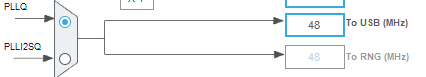
\includegraphics[width=0.5\linewidth]{Figures/usb_clock_config.png}
        \caption[  USB clock frequency]{The clock frequency of the USB}
        \label{fig:clock_usb}
    \end{figure}

    To make it possible for the receiver script to detect the start of each data packet, a two-byte synchronization word was added before the audio payload, as shown in Code~\ref{lst:usb_sync}.\\

    \begin{lstlisting}[style=cstyle, caption={Bytes used for syncing the data packages}, label={lst:usb_sync}]
    #define USB_SYNC_0            0x5A
    #define USB_SYNC_1            0xA5
    \end{lstlisting}

    \newpage
    The PCM values in the two-byte format are transfered to the receiver script by using the \textbf{PackAndSendFrame} function in \textbf{main.c} of the MCU program. The function is called in the \textbf{While} loop visible in the Code~\ref{lst:while_loop_c}, when all of the filter buffers were either half-full og completly full. The function itself can be seen in Code~\ref{lst:pack_and_send}, and its main task is to transfer 16 samples from each DMA filter buffer to a separate container, and place it into a frame. The packed frame is later send through the \textbf{CDC\_Transmit\_FS} method to the receiver script.\\

\begin{lstlisting}[style=cstyle, caption={Main loop for checking DMA buffer readiness and transmitting audio frames}, label={lst:while_loop_c}]
     while (1)
  {
	      if (flt0_half_ready && flt1_half_ready && flt2_half_ready && flt3_half_ready)
	      {
	          flt0_half_ready = 0;
	          flt1_half_ready = 0;
	          flt2_half_ready = 0;
	          flt3_half_ready = 0;
	          PackAndSendFrame(0);
	      }
	      if (flt0_full_ready && flt1_full_ready && flt2_full_ready && flt3_full_ready)
	      {
	    	  flt0_full_ready = 0;
	    	  flt1_full_ready = 0;
	    	  flt2_full_ready = 0;
	    	  flt3_full_ready = 0;
	          PackAndSendFrame(1);
	      }
  }
\end{lstlisting}
    \begin{lstlisting}[style=cstyle, caption={Function for packing and sending each frame, generated by \cite{chatgpt2026}}, label={lst:pack_and_send}]
    static void PackAndSendFrame(uint8_t half_index)
{
    uint32_t start = (half_index == 0) ? 0 : PCM_SAMPLES_PER_HALF;
    usb_frame[0] = USB_SYNC_0;
    usb_frame[1] = USB_SYNC_1;
    uint32_t j = 2;
    for (uint32_t i = 0; i < PCM_SAMPLES_PER_HALF; i++)
    {
        int16_t mic0 = DFSDM32_to_PCM16(pcm0_dma[start + i]);
        int16_t mic1 = DFSDM32_to_PCM16(pcm1_dma[start + i]);
        int16_t mic2 = DFSDM32_to_PCM16(pcm2_dma[start + i]);
        int16_t mic3 = DFSDM32_to_PCM16(pcm3_dma[start + i]);
        
        usb_frame[j++] = (uint8_t)(mic0 & 0xFF);
        usb_frame[j++] = (uint8_t)((mic0 >> 8) & 0xFF);
        usb_frame[j++] = (uint8_t)(mic1 & 0xFF);
        usb_frame[j++] = (uint8_t)((mic1 >> 8) & 0xFF);
        usb_frame[j++] = (uint8_t)(mic2 & 0xFF);
        usb_frame[j++] = (uint8_t)((mic2 >> 8) & 0xFF);
        usb_frame[j++] = (uint8_t)(mic3 & 0xFF);
        usb_frame[j++] = (uint8_t)((mic3 >> 8) & 0xFF);
    }
    CDC_Transmit_FS(usb_frame, sizeof(usb_frame));
}
void CDC_TransmitCplt_FS(uint8_t *Buf, uint32_t *Len, uint8_t epnum)
{
    (void)Buf;
    (void)Len;
    (void)epnum;
    usb_tx_busy = 0;
}
\end{lstlisting}
\subsection{Data Acquisition and Communication}
The data from the microhpones was transmitted in the PDM format, and acquired by the DFSDM peripheral. After filtering and decimatiion in the DFSDM, the resulting PCM samples were transmitted to the PC through USB CDC. 

    \subsubsection{PDM input from digital MEMS microphones}
    The digital MEMS microhpones output a PDM bitstream, where the data rate is controlled by the clock signal applied to  the \textbf{CLK} pin. In the project, the clock signal was generated by the DFSDM peripheral and set to 2 Mhz, which is right between the necessery signal frequency of 1.2 Mhz to 3.25 Mhz according to \cite{st_mp34dt06j_2021}. The resulting PDM stream varies according to the acoustic pressure measured by each microphone and was used as the input to the DFSDM channels. 

    \subsubsection{PDM to PCM conversion with DFSDM}
    The PDM samples are converted to PCM format by the DFSDM peripheral, which uses the sinc filter of the 3rd order and decimates the values by the ratio of 32. The newly converted samples are then stored in a 32-bit word, which are furtherly converted to the \textbf{int16\_t} format to reduce the maximal value of each sample as seen in Code~\ref{lst:pack_and_send}.   
    
    \begin{lstlisting}[style=cstyle, caption={Limiting the shifted DFSDM output to the valid signed 16-bit PCM range. Generated by \cite{chatgpt2026}.}, label={lst:pack_and_send}]
    static int16_t DFSDM32_to_PCM16(int32_t x)
    {
        x >>= 8;
    
        if (x > 32767)  x = 32767;
        if (x < -32768) x = -32768;
        return (int16_t)x;
    }
    \end{lstlisting}
    \subsubsection{PCM samples}
    Each microphone is expected to provide 16 PCM samples per iteration after the conversion from PDM to PCM. The reason for that, is the earlier application of SAI and pdm2pcm library, where the user had to specify the number of output samples and the decimation rate. Where by using the decimation rate of 64, and the PCM samples number of 16 togheter with the clock signal, the user was then able reach the desired Fs of around 24Khz per second. So to not chagne the later pipeline involving the receiver script, the number of samples was not changed.  

    
    \newpage
    \subsubsection{PCM sample format sent by the usb}
        \label{sec:PCM_sample_format_sent_by_usb}
        The MCU sends the PCM samples in frames of the format that can be seen in Table~\ref{tab:usb_frame_structure}. Each frame starts with a two byte synchonization word, followed  by the adio payload. The payload contains 16 PCM samples from each mirophone and since each PCM sample is stored as an \textbf{int16\_t} value, each sample requires 2 bytes. That gives 32 data bytes per microphone channel and 128 bytes of the data payload in total. By adding the two sync bytes, the total frame length becomes 130 bytes. 
        
\begin{table}[h]
\centering
\caption{USB frame structure}
\label{tab:usb_frame_structure}
\begin{tabular}{|c|c|c|c|}
\hline
\textbf{Field} & \textbf{Size} & \textbf{Content} & \textbf{Description} \\
\hline
Sync word & 2 bytes & 0x5A 0xA5 & Marks the start of a new frame \\
\hline
Audio payload & $16 \times 4 \times 2$ bytes & PCM samples & 16 samples per microphone \\
\hline
Total frame & 130 bytes & Sync + payload & Complete USB frame sent to Python \\
\hline
\end{tabular}
\end{table}

\subsection{The main python program for the signal processing}
The part of the system responsible for the signal processing of the acoustic signal, sound source estimation and the feature extraction is controlled by the \textbf{main.py} file found in the \textbf{Drone\_detection\_porgram\_bachelor/} folder. The program pipeline can be seen in the Figure~\ref{fig:main_flowchart}. The program initializes the following objects Code~\ref{lst:init_main_py}, which are responsible for receiving the microphone signal, estimating the source of the incoming signal and also extraction of the features present in the signal, that can be later used in the ML based classifier.

\begin{lstlisting}[style=pythonstyle, caption={Initialization of the objects used in the main.py}, label={lst:init_main_py}]
from receivers.stm32_usb_receiver import STM32UsbReceiver
from dataset_tools.create_wav_file import WavCreation
from features.mfcc_extraction import  MFCCExtractor
from features.feature_exporter import FeatureExporter
from features.feature_visualizer import FeatureVisualizer
from debug.stm32_usb_receiver_debug_tools import ReceiverDebug
from gcc.gcc_processor import GCCProcessor
from gcc.doa_estimator import DOAEstimator
from gcc.doa_visualizer import DOAVisualizer

receiver = STM32UsbReceiver()
wav_conversion = WavCreation()
mfcc_extractor = MFCCExtractor()
mfcc_exporter = FeatureExporter(extractor=mfcc_extractor)
mfcc_visualizer = FeatureVisualizer(extractor=mfcc_extractor)
gcc_processor = GCCProcessor()
doa_estimator = DOAEstimator(p_vector, gcc_processor)
doa_visualizer = DOAVisualizer()
#debug 
receiver_debug = ReceiverDebug(receiver=receiver)
\end{lstlisting}

\newpage
\begin{figure}[h]
    \centering
    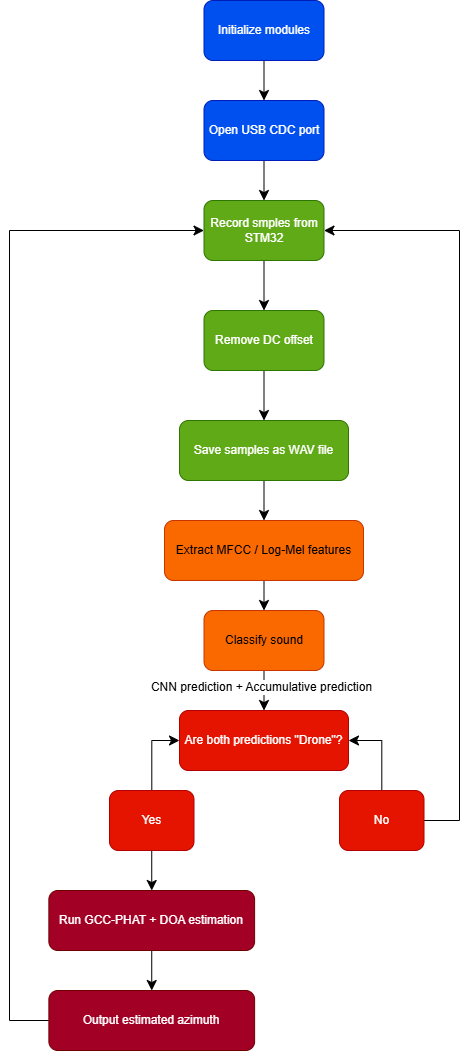
\includegraphics[width=0.5\linewidth]{Figures/main_program.drawio.png}
    \caption[  Flowchart-main program for audio]{Flowchart for the main program for audio processing }
    \label{fig:main_flowchart}
\end{figure}
The program runs continuously, as it is based on a while loop, which can be modified to either run infinitely, or for a set number of iterations. The program loop used during the system testing can be seen in Code~\ref{lst:while_main}.
\newpage
\begin{lstlisting}[style=pythonstyle, caption={The main program loop for sound detection and classification}, label={lst:while_main}]
while Run:
    i+=1
    samples = receiver.record() # record the data sent by the stm32
    # test DC offset 
    samples= samples.astype(np.float32)
    samples = samples - np.mean(samples)

    wav_conversion.convert_into_wav(samples, receive_time=receiver.start_time, duration= receiver.duration_sec) # convert the samples into a wav format
    receiver_debug.debug_export(plot_debug=True)

    # features 
    features = mfcc_extractor.extract_features(audio_file=f"debug_figures/04_05_drone_test_riktig_plassering/mic_recording{receiver.start_time}.wav") # extract features such as mfcc, delta, delta2, log_mel_spec etc
    mfcc_exporter.df_features() # export the features into a df
    # adds a lot of overhead, comment out during live testing
    #mfcc_visualizer.mel_spectrogram(receiver.start_time)
    #mfcc_visualizer.spectrogram(receiver.start_time)
    
    # Sound classification
    cnn_predict = cnn_model.cnn_predict(f"debug_figures/04_05_drone_test_riktig_plassering/mic_recording{receiver.start_time}.wav") #Fix, add permanent non debug location
    accumulative_predict = accumulative_model.acum_predict(features)
    
    if cnn_predict == "Drone" and accumulative_predict == "Drone":
        # Direction
        gcc_array = gcc_processor.process_signal(samples, mfcc_extractor.fs)
        doa_estimator.set_gcc_array(gcc_array)
        doa_estimator.estimate_DOA()
        print(f"Azimuth this iteration is: {doa_estimator.estimated_azimuth_deg}")
        print(f"Iteration: {i}")
        # adds a lot of overhead, comment out during live testing
        #doa_visualizer.visualize_doa(doa_estimator.estimated_azimuth_deg, doa_estimator.estimated_azimuth_rad, #receiver.start_time)
        
    if i == 45: # allows for 45 iterations, before the program terminates
        Run = False   
    # debug 
    print(f"CNN prediction: {cnn_predict}")
    print(f"Accumulative prediction: {accumulative_predict}")
    
    if debug_mfcc:
        mfcc_visualizer.plot_signal_time()
        mfcc_visualizer.spectrogram()
        mfcc_visualizer.mel_spectrogram()
        Run = False
    if debug_stm32:
        receiver_debug.debug_export(plot_debug=True)
        Run = False 
\end{lstlisting}

During each iteration, the new samples are measured, by calling the \textbf{record} member function of the receiver object. Then the DC offset is subtracted from the signal, to center the signal around zero. The measured signal has to be converted into a wav sound file, which is the needed signal format for the MFCC extraction class. The signal features are then extracted by using the \textbf{extract\_features} from the MFCC extractor type object, which will later be send to the ML classifier to decide what kind of the object is producing the sound. But before that the direction of the source signal will be estimated, and the program will then determine based on the classifiers output, to either keep the estimated azimuth or to find a new one that correclty represents drone signal source. The program uses also some debug functions, which were extensively used during the testing stage of the project.  


\subsection{Python receiving and preprocessing}
The PCM signal transmitted by the MCU to the host computer is first handled by a Python receiving module, placed in the \textbf{Drone\_detection\_porgram\_bachelor/receivers} folder, called \textbf{stm32\_usb\_receiver.py}. The module decodes the incoming USB frames and prepers the microphone singal for the later processing stages such as direction estimation and feature extraction. 

    \subsubsection{USB CDC receiver}
    The receiver object was initialized using the configuration shown in Table~\ref{tab:receiver_config}. The parameters are used to define the USB port, the expected synchronization word, the number of microphones, samples per microphone, the duration time of the recording and the number of expected bytes in the frame.

    \begin{table}[h]
\centering
\caption{Configuration parameters used by the STM32 USB receiver}
\label{tab:receiver_config}
\begin{tabular}{|c|c|c|}
\hline
\textbf{Parameter} & \textbf{Value} & \textbf{Description} \\
\hline
\texttt{port} & \texttt{COM16} & USB CDC port used on Windows \\
\hline
\texttt{sync} & \texttt{0x5A 0xA5} & Two-byte synchronization word \\
\hline
\texttt{channels} & 4 & Number of microphone channels \\
\hline
\texttt{frame\_samples} & 16 & Number of samples per microphone in each frame \\
\hline
\texttt{duration\_sec} & 1 & Recording duration for each iteration \\
\hline
\texttt{frame\_bytes} & 130 & Expected size of one complete USB frame \\
\hline
\end{tabular}
\end{table}
    The receiver class contains methods for opening and closing the USB CDC port, but the main processing is performed by the \textbf{record()} method which can be seen in Code~\ref{lst:record_method}. 
    \newpage
    \begin{lstlisting}[style=pythonstyle, caption={Record the signal method. Was originally generated by \cite{chatgpt2026}, but was modified during the debuging process}, label={lst:record_method}]
    def record(self):
        # remove old data, initiate a temp buffer
        if self.port_opened:
            self.ser.reset_input_buffer() 
            rx_buf = bytearray()

            print("Recording..")
            self.start_time = time.time()
            self.samples = [[] for _ in range(self.channels)] #reset the samples before recording any new values
            
            while time.time() - self.start_time < self.duration_sec :
                data = self.ser.read(512) # 512 bytes
                
                if not data:
                    continue
                rx_buf.extend(data) # adds data to rx_buf

                while True:
                    sync_idx = rx_buf.find(self.sync) 

                    if sync_idx < 0: # if sync was not in the buffer
                        # keep the last byte in case sync 2 bytes are divided between packages
                        rx_buf = rx_buf[-1:]
                        break

                    if len(rx_buf) < sync_idx + self.frame_bytes:
                        # if the length of data is smaller then the expected frame length plus sync bytes
                        break

                    frame = rx_buf[sync_idx + 2 : sync_idx + self.frame_bytes]
                    rx_buf = rx_buf[sync_idx + self.frame_bytes:] # removes the processed frame 

                    samples = np.frombuffer(frame,dtype=np.int16) # interpret as signed int16
                    
                    # vectorized 
                    samples = samples.reshape(-1, self.channels)
                    self.samples = [np.concatenate((self.samples[ch], samples[:,ch])) for ch in range(self.channels)]
    
            return np.array(self.samples)

        else:
            raise RuntimeError("THE PORT WAS NOT OPENED! Use open_port().")

        \end{lstlisting}
    
     The method after opening the port, zeroes out the samples for each channel connected to the object, insuring that only the data from the current iteration will be processed. The data is being gathered for a default duration of 1 second, during which the package is controlled for the sync bytes. If the sync bytes are not present in the package, the receiver keeps the last byte and waits for more of the incoming data, in case the sync word was splitt between two reads. If the sync bytes are found, but the buffer does not yet contain the complete 130 bytes frame, the receiver also waits for more data before processing the frame. After the complete frame has been extracted, the sync bytes are removed, and the remaining data is then stored in the \textbf{frame} container. In its current format, the payload is still just a byte-string, which has to be interpreted as 16-bit integer values to reconstruct the PCM values. Since the payload sent from the MCU is interleaved, each sample index contains one sample from each microphone in the order mic0, mic1, mic2 and mic3. The payload is therefore reshaped into four colums, where each represents an independent microphone signal.   
    
    \subsubsection{DC offset removal}
    The DC offset removal was conducted in the \textbf{main.py} in Code~\ref{lst:DC_Offset}, by converting the values inside of the \textbf{samples} containter into the \textbf{float32} format to insure that the function \textbf{np.mean()} can be applied. Then the mean value of the signal was subtracted from the samples. This removes the value that the signal is circulating around as seen in Figure~\ref{fig:DC_offset} and effectively centers the values around zero . 

    \begin{lstlisting}[style=pythonstyle, caption={DC offset romoval}, label={lst:DC_Offset}]
    # test DC offset 
    samples= samples.astype(np.float32)
    samples = samples - np.mean(samples)
    \end{lstlisting}

    \begin{figure}[h]
    \centering
    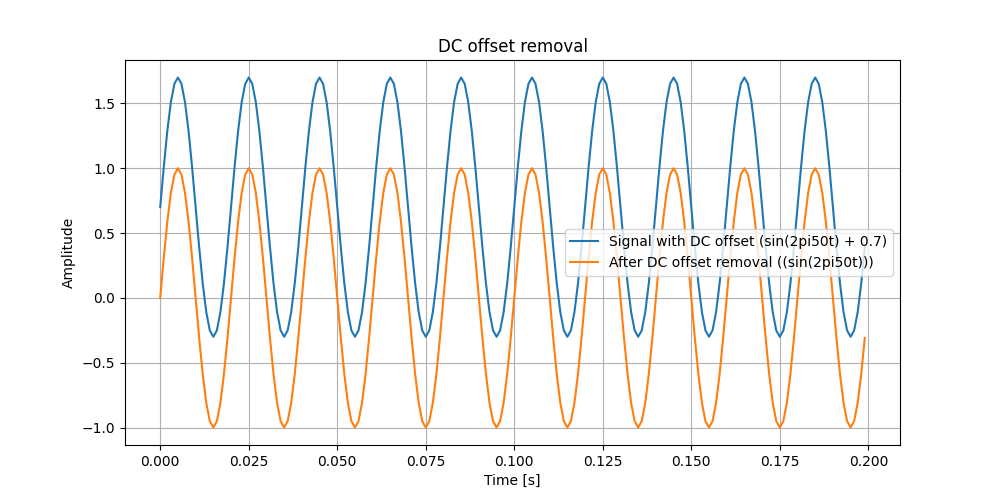
\includegraphics[width=0.7\linewidth]{Figures/dc offset removal.png}
    \caption[  DC offset comparison]{Comparison of the signal with a DC offset of 0.7, and the signal with the DC offset removed.}
    \label{fig:DC_offset}
    \end{figure}
    \newpage
    \subsubsection{WAV file generation}
    The measured and offset signal before the further analysis, has to be converted to a \textbf{.wav} type file. The main reason for that was the use of the sound file in the debuging and testing process, and the possibility to use some of the member functions present in the \textbf{librosa} library, which was extencively used in the feature extraction process. The code responsible for the conversion of the signal can be seen in Code~\ref{lst:wav_file}.

\begin{lstlisting}[style=pythonstyle, caption={Class for the conversion of the signal to the wav file.}, label={lst:wav_file}]
from scipy.io.wavfile import write
from receivers.stm32_usb_receiver import STM32UsbReceiver
import numpy as np

class WavCreation:
    """
    Creates the wav sound file, using samples gathered with 
    stm32_usb_receiver
    
    Has one func called convert_into_wav(), that write the sound file into recordings folder. 
    """
    def __init__(self):
        pass

    def convert_into_wav(self, samples : np.ndarray, receive_time : STM32UsbReceiver, duration : STM32UsbReceiver):
        filename =f"debug_figures/04_05_drone_test_riktig_plassering/mic_recording{receive_time}.wav"
        effective_fs = len(samples[0])/ duration
        #print([len(ch) for ch in samples])
        #print(samples.shape)
        #print(samples.dtype)
        #print(effective_fs)
        audio = np.stack(samples, axis=1)
        audio = np.clip(audio, -32768, 32767).astype(np.int16)
        write(filename,int(round(effective_fs)), audio)

\end{lstlisting}  

\newpage
\subsection{Feature Extraction}
    The feature extruction is conducted by calling the \textbf{extract\_features()} which is an external method of the feature extraction class that can be accesed in \textbf{Drone\_detection\_porgram\_bachelor/features/mfcc\_extraction.py}. The class was initialized with the parameters shown in Table~\ref{tab:mfcc_parameters}. The feature extraction method is mainly based on the ideas taken from (\cite{singh2014mfcc} and \cite{zheng2001mfcc}).

    \begin{table}[h]
\centering
\caption{Parameters used in the MFCCExtractor class}
\label{tab:mfcc_parameters}
\begin{tabular}{|c|c|c|}
\hline
\textbf{Parameter} & \textbf{Value} & \textbf{Description} \\
\hline
\texttt{n\_mfcc} & 40 & Number of MFCC coefficients \\
\hline
\texttt{n\_fft} & 1024 & FFT size used for spectral analysis \\
\hline
\texttt{hop\_length} & 250 & Number of samples between consecutive frames \\
\hline
\texttt{win\_length} & 500 & Window length used for each frame \\
\hline
\texttt{n\_mels} & 40 & Number of Mel filters \\
\hline
\end{tabular}
\end{table}
    
    The \textbf{extract\_features()} returns the accumulated features representing the spectral behaviour of the signal, and can be seen in Code~\ref{lst:extract:features}. The function is based on the internal methods, that were used to simplify the process of extracting the spectral features of the measured signal.

    \begin{lstlisting}[style=pythonstyle, caption={Definition of the extract\_features method.}, label={lst:extract:features}]
    def extract_features(self, audio_file):
        self._convert_wav_to_signal(audio_file)
        self._mfcc_after_preemphasis()
        self._create_mel_spec()
        self._power_mel_spec()
        self._accumulate_the_stats()
        return self.acc_features
    
    \end{lstlisting}
    \newpage
    \subsubsection{Extraction pipeline}
    The feature extraction pipeline, can be seen in Figure~\ref{fig:mfcc_pipeline}, which describes how the features are extructed and then exported. 
    
    \begin{figure}[h]
        \centering
        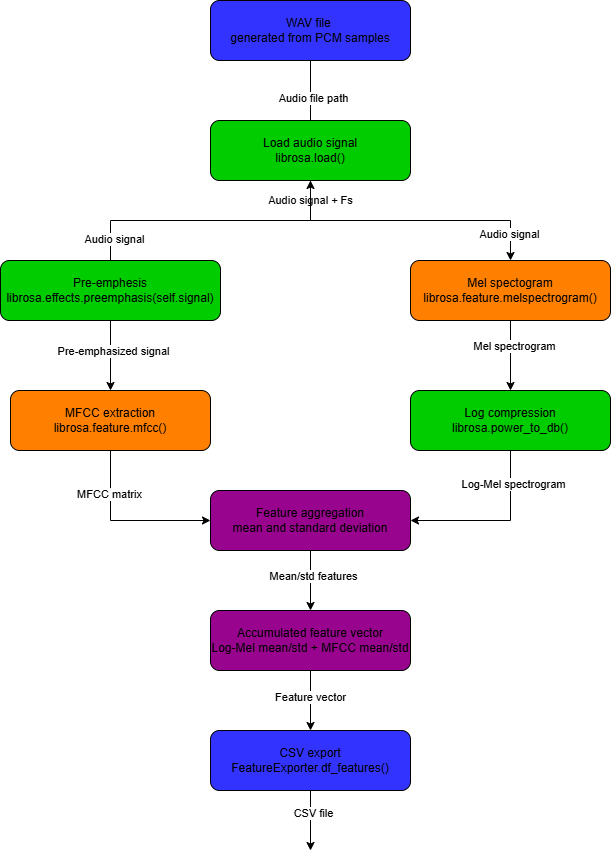
\includegraphics[width=0.48\linewidth]{Figures/mfcc_pipeline.png}
        \caption[  Flowchart- feature extraction]{Feature extraction pipeline}
        \label{fig:mfcc_pipeline}
    \end{figure}
    
    \subsubsection{Wav conversion}
    The first stage of the feature extraction process is conducted in the\\
    \textbf{\_convert\_wav\_to\_signal()}, which uses the \textbf{.load()} function from the Librosa library. The .load() function, process the wav file and converts it into an array representing the signal, and also returns a scalar representing the signals FS. The functions declaration can be seen in Code~\ref{lst:wav_to_signal}.

    \begin{lstlisting}[style=pythonstyle, caption={The function used to convert the wav file into an array of samples}, label={lst:wav_to_signal}]
    def _convert_wav_to_signal(self, audio_file):
        self.signal, self.fs = librosa.load(audio_file, sr = None)
        self.signal_time_domain = self.signal
    \end{lstlisting}
    
    \subsubsection{Pre-emphesis}
        The pre-emphesis was conducted by applying a method from the librosa library, which is based on the following filter design Equation~\ref{eq:n-order_diff_filter}], which represents the first-order differencing filter (\cite{librosaPreemphasis}). The pre-emphesis was applied to amplify the high frequency components present in the signal, by using the default settings in the Librosa method, such as coef being equal 0.97.

    \begin{equation}
        \label{eq:n-order_diff_filter}
        y[n] -> y[n] - coef*y[n-1]
    \end{equation}

    \subsubsection{MFCC extraction}
    \raggedbottom
    In the project the MFCC are used to describe the overall spectral shape of the measured acoustic signal.
    The extraction of the mfcc is conducted in \textbf{\_mfcc\_after\_preemphesis()} seen in Code~\ref{lst:mfcc_function}, which takes the pre-emphasised signal and the sampling frequency, and uses them as the base of the feature extraction. The extraction itself is conducted by applying the \textbf{feature.mfcc()} method taken from librosa, which uses the values initializing the class object as in the Table~\ref{tab:mfcc_parameters}.\\
    \begin{lstlisting}[style=pythonstyle, caption={Function used for the mfcc extraction}, label={lst:mfcc_function}]
    def _mfcc_after_preemphasis(self):
        signal_preemphasised = self._get_preemphasised_signal()

        self.mfcc = librosa.feature.mfcc(
            y = signal_preemphasised,
            sr = self.fs,
            n_mfcc= self.n_mfcc,
            n_fft = self.n_fft,
            hop_length = self.hop_length,
            win_length = self.win_length,
            n_mels = self.n_mels
        )
    \end{lstlisting}
    Beside the pre-emphasized signal and its sampling frequency, the method uses the following arguments:\\
    \begin{enumerate}
        \item \textbf{n\_mfcc} - represents the number of coefficients used to describe the spectrum present in each frame. The higher number of coefficients allows for a wider representation of the spectrum, but at the same time increases the computational time needed to extract the spectral information, represented by each coefficient. The value used in the project is 40, which gave accurate enough representation of the spectrum, without much of a time delay.\\
    \item \textbf{n\_fft} - represents the number of points used for the frequency analysis of the signal. The higher the value the lower the spacing between the frequency bins, allowing for more accurate representation of the energy division between the frequency components. The value used in the project is 1024, which in combination with the Fs of around 20 Khz, gives around 19.5 Hz per frequency bin.\\
    \item \textbf{hop\_length} - defines the sample distance between the consecutive frames. In this project, the length of 250 samples was used, which divided by the Fs of 20 Khz, gives around 12.5 ms between each frame. The reason for the use of that particular number, was the assumption of 50\% overlap between the frames, where each frame is expected to hold 500 samples.\\
    \item \textbf{win\_length} - represents the number of samples present in each frame, where each frame has to represent around 25 ms. To find the number of samples needed to represent the time period of 0.025 seconds, the desired period has to be multiplied by Fs of 20 Khz which gives 500 samples.
    \item  \textbf{n\_mels} - represents the number of Mel-scaled band-pass filters, which are applied to the signal to convert it into Mel frequency spectrum. The number of the filters used is 40, which is two times the number of filters used in (\cite{singh2014mfcc}), to increase the details of the signal. 
    \end{enumerate}

    After the extraction the MFCC are saved in the extraction object. 
    
    \subsubsection{Log-Mel spectrogram}
    In the project, the log-mel spectrograms are used to describe the energy distribution across the Mel-frequency bands over time. 
    The Mel spectrogram is generated using the \textbf{librosa.feature.melspectrogram()} method, which uses the same frame-based parameters as the MFCC extraction method. To obtain the  logharitmic representation of the spectral energy, the \textbf{librosa.power\_to\_db()} method is applied. The Log-Mel spectrogram was extracted because it represent the energy distribution of the signal across the Mel-frequency bands, which allows to describe where in the Mel-frequency spectrum most of the signal energy is located.
    
    \subsubsection{Feature aggregation}
    The features from the MFCC and Log-mel spectrogram are being accumulated to create a fixed-size feature vector for each recorded signal. This is necessary because both methods return values based on the analysis frame, where each frame contains a set of MFCC coeffieicents or Mel-frequency band energies. The total number of frames will change, if the recording is shortened due to any microphone mulfunction present, which could introducce a situation where one recording is represented by fewer frames then the previous one. This could make the signal incompatible with the classifier, as it expects a fixed-size feature vectors. Hence the features are aggregated by taking a mean and standard deviation (std) of the Log-Mel and MFCC coefficients. The mean value of the Log-Mel represents the average energy distribution, while the mean of the MFCC represents the average spectral shape. The std of the MFCC shows how the whole spectrum changes over time, while the std of the Log-Mel, represents how much enregy in each band changes over time. The funtion responsible for the aggregation is called \textbf{\_accumulate\_the\_stats} and can be seen in Code~\ref{lst:accumulate_the_stats}.
    
    \begin{lstlisting}[style=pythonstyle, caption={Function used for feature accumulation}, label={lst:accumulate_the_stats}]
    def _accumulate_the_stats(self):
        # mffcc mean - avg spectral shape, or how the sound looks like in the spectrum. Is it more "flat" or "steep" or "curved"
        # mfcc std - how much the whole spectral envelope changes over time 

        # log-mel mean - how the energy is distirbuated across freq bands (in db)
        # low-mel std - how much energy in each band changes over time

        logmel_stats = np.hstack([self.log_mel_spec.mean(axis=1), self.log_mel_spec.std(axis=1)])
        mfcc_stats = np.hstack([self.mfcc.mean(axis=1),self.mfcc.std(axis=1)])
        self.acc_features = np.hstack([logmel_stats,mfcc_stats])
    \end{lstlisting}

    
\subsection{Direction of arrival estimation (DOA)}
The direction of arrival estimation of the detected drone was conducted by using the\\ \textbf{gcc\_processor.py} and \textbf{doa\_estimator.py} modules. The flow chart for the TDOA estimation pipeline can be seen in Figure~\ref{fig:doa_estimation}. The method is mainly a mix of ideas taken from (\cite{kwon2010gccphat}, \cite{kang2016prefiltering} and \cite{blandin2012multisource}). 

\begin{figure}[h]
    \centering
    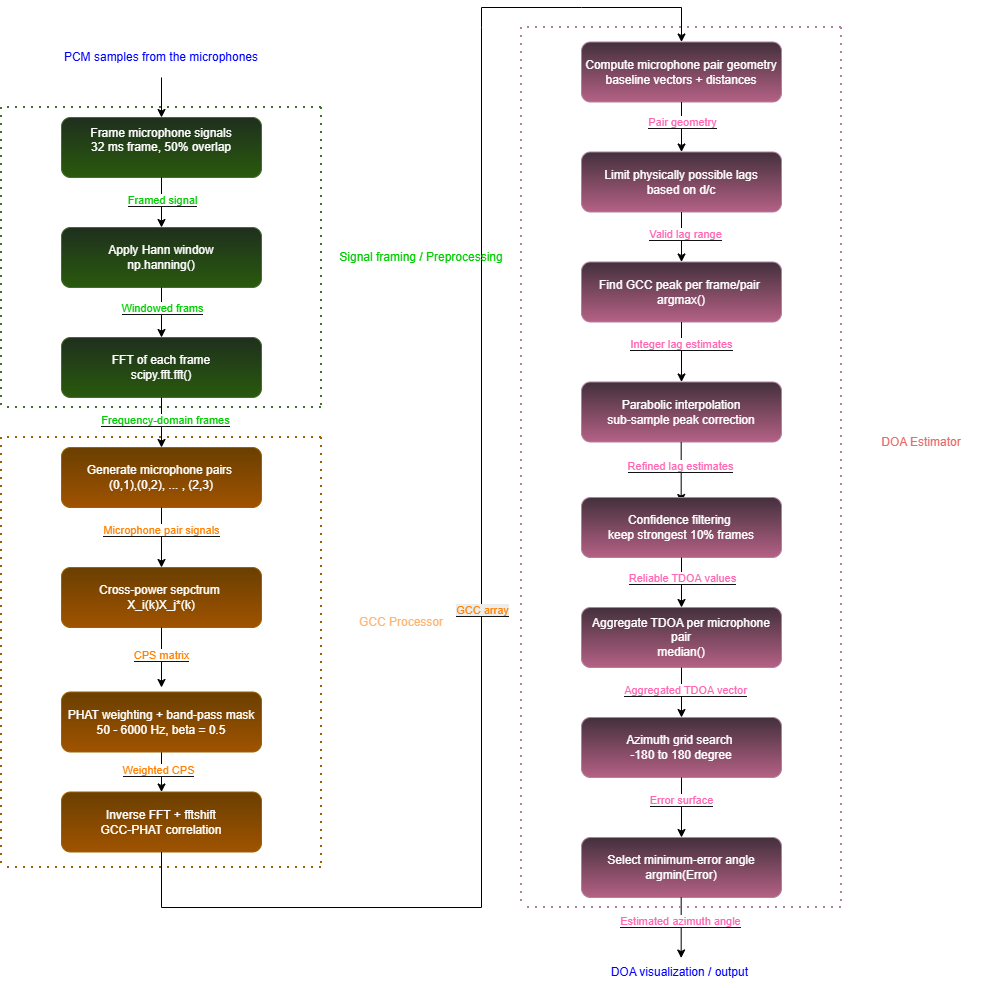
\includegraphics[width=0.6\linewidth]{Figures/gcc_flow_chart.drawio (5).png}
    \caption{DOA estimation pipeline}
    \label{fig:doa_estimation}
\end{figure}


    \subsubsection{GCC processor}
    The gcc\_processor module processes the microphone signals in pairs by framing the signals, applying a window function, calculating the FFT, and computing the cross-power spectrum between each microphone pair. The CPS is then weighted using the PHAT method, and transformed back to the time doamin the GCC-PHAT correlation function (\cite{kwon2010gccphat}). To produce the weighted CPS values, the \textbf{process\_signal} function as seen in Code\ref{lst:process_signal}, has to called with the measured signal as an argument.\\

    \begin{lstlisting}[style=pythonstyle, caption={Function used to produce the correlation matrix of the microphone.}, label={lst:process_signal}]
    def process_signal(self, samples: np.ndarray, fs): #samples has to be np.array to use .shape
        self.fs = fs
        samples_per_frame = int(self.fs * self.frame_ms / 1000)
        frames = self._frame_samples(samples, samples_per_frame)
        windowed_frames = self._window_each_frame(frames)
        frames_fft = self._fft_each_frame(windowed_frames)
        cps_array = self._cross_power_spectrum(frames_fft)
        gcc_array = self._p_hat_weighted_gcc(cps_array, fs, samples_per_frame)
        return gcc_array
    \end{lstlisting}    
    
    \paragraph{Signal framing}
    The signal framing is done in the \textbf{\_frame\_samples} method, which can be seen in Code~\ref{lst:frame_sample_gcc}. The reason for the framing application is the same as for the framing of the signal for the MFCC, namely the need of representing the signal as stationary for the application of FFT. \\

    \begin{lstlisting}[style=pythonstyle, caption={Function used for signal framing for gcc.}, label={lst:frame_sample_gcc}]
    def _frame_samples(self,samples: np.ndarray, samples_per_frame):
        if samples is not None:
            frames = []
            samples_n = samples.shape[1]
            hop = samples_per_frame//2
            for frame_n in range(int(samples_n/hop)):
                start = frame_n * hop
                end = start + samples_per_frame

                if end <= samples_n:
                    frames.append(samples[:, start:end])
            return np.array(frames)
        else:
            raise RuntimeError("No samples present, gather them again")
    \end{lstlisting}
    \newpage
    \paragraph{Windowing}
    The windwing is conducted to reduce the effects of the spectral leakage. The function \textbf{\_window\_each\_frame()} does so by using the \textbf{hanning} from the numpy library, which multiplies the signal by the hann window function, resulting in a signal with reduced spectral leakage. The function was applied as seen in Code~\ref{lst:window_gcc}.\\

    \begin{lstlisting}[style=pythonstyle, caption={Function used for windowing the signal.}, label={lst:window_gcc}]
    def _window_each_frame(self,frames: np.ndarray):
        hanning = np.hanning(int(frames.shape[-1]))
        windowed_frames = frames * hanning
        return windowed_frames
    \end{lstlisting}
    
    \paragraph{FFT and cross-power spectrum}
    The CPS is found by calling the \textbf{\_cross\_power\_spectrum()} function, which expects to receive the frames in the frequency-domain. The transformation of the time-domain frames into the frequency domain is conducted by using the \textbf{\_fft\_each\_frame()} method. The FFT of one microphone signal is later multipplied by the complex conjugate of the FFT of the other microphone signal as introduced in the theory section. The microphone pairs were generated by using the \textbf{\_generate\_mic\_pairs()}, which returns all unique microphone pair combinations. For four microphones, this results in six microphone pairs. The methods used for the FFT, pair generation and the CPS calculations are shown in Code~\ref{lst:fft_and_cps}.\\

    \begin{lstlisting}[style=pythonstyle, caption={Functions used to fing the CPS of the microphone pair, before the PHAT weighting.}, label={lst:fft_and_cps}]
    def _fft_each_frame(self,frames):
        frames_frq_domain = fft(frames, axis=-1)
        return frames_frq_domain
    
    def generate_mic_pairs(self, n_mics): # is quite needed in the tdoa and doa
        return [(i,j) for i in range(n_mics) for j in range(i+1, n_mics)]

    def _cross_power_spectrum(self,frames_fft:np.ndarray):
        # try to vectorize?
        # use list comprahension?
        cps = []
        n_frames = frames_fft.shape[0]
        n_mics = frames_fft.shape[1]
        self.n_mics = n_mics

        if self.mic_pairs is None:
            self.mic_pairs = self.generate_mic_pairs(n_mics)
        
        mic_pairs = self.mic_pairs

        # for each frame multi mic_i with the conjugate of mic_j

        for frame in range(n_frames): 
            frame_cps = [] # cps of one frame
            for i,j in mic_pairs:
                cps_ij = frames_fft[frame, i, :] *frames_fft[frame,j,:].conj()
                frame_cps.append(cps_ij)
            cps.append(frame_cps)

        # frame_cps shape (frame, mic pair, cps)
        return np.array(cps)
        \end{lstlisting}
    
    \paragraph{PHAT weighting}
    After the CPS between the microphones was estimated, the PHAT weighting has to be applied to reduce the influence of high-amplitude frequency components, which is accomplished by calling the\\
    \textbf{\_p\_hat\_weighted\_gcc()} function. Inside of the method, the CPS values are divided by CPS magnitude raised to the power of $\beta$, as introduced in the theory part based on (\cite{kang2016prefiltering}). To the magnitude of the CPS, the epsilon of 1e-13 was also added, to avoid the division by zero. The scaling value of $\beta$ used in the project is 0.5, which was chosen to be an initial testing value, before the application of the SNR based $\beta$ value estimation. After the weighting was conducted, the CPS values are also filtered by a frequency mask of frequency interval of 80 Hz to 6000 Hz. The frequency for the frequency mask was chosen long before the testing on the live drone was conducted. The weighted CPS values are then transformed back to the time-domain, where they represent the correlation between the microphones over the possible time lags. The result is then shiftet to be centered around zero. The declaration of function used can be seen in Code~\ref{lst:phat_weighting}.\\

    \begin{lstlisting}[style=pythonstyle, caption={Function used to weight the CPS values.}, label={lst:phat_weighting}]
    def _p_hat_weighted_gcc(self,cps_array :np.ndarray, fs, n_samples_per_frame, freq_low = 80, freq_high = 6000, beta = 0.5, eps = 1e-13, use_adaptive_beta = False ):
        freq = np.fft.fftfreq(n_samples_per_frame, d = 1/fs) # array of freq for each fft bin
        band = (freq_low <= np.abs(freq)) & (np.abs(freq) <= freq_high) # boolean mask to remove unwanted freq
        mag = np.abs(cps_array) + eps
        
        weighted_cps = cps_array/(mag**beta)
        weighted_cps *= band 
        gcc_array = np.fft.ifft(weighted_cps, axis =-1)
        gcc_array = np.fft.fftshift(gcc_array, axes = -1)

        return np.real(gcc_array)
    \end{lstlisting}


        
    \subsubsection{DOA estimator}
    The doa\_estimator uses resulting time-delay information from the microphone pairs and compares it with simulated TDOA values for different azimuth angles. The azimuth angle with the best match is then selected as the estimated DOA of the sound source. The code responsible for the DOA estimation, can be seen in Code~\ref{lst:doa_estimation}.

    \begin{lstlisting}[style=pythonstyle, caption={Function used to estimate the DOA}, label={lst:doa_estimation}]
     def estimate_DOA(self):
        self._compute_pair_geometry()
        self._compute_lags_per_pair()
        self._estimate_tdoa()
        self._estimate_azimuth()
    \end{lstlisting}
    \newpage
    \paragraph{Pair geometry}
    For the system to properly estimate direction of the sound source, the baseline vector and the norm of each microphone pair has to be computed.
    The baseline vector describes the relative position between the two microphones and is found by subtracting one microphone position from the other. The norm gives the physical distance between the microphones, which is later used to calculate the maximum possible time delay for each pair. The baseline vectors and norms are computed by calling \textbf{\_compute\_pair\_geometry()}, as shown in Code~\ref{lst:pair_geometry}.\\  

    \begin{lstlisting}[style=pythonstyle, caption={Function used to compute the pair geometry.}, label={lst:pair_geometry}]
    def _compute_pair_geometry(self):
        # Finds the baseline vectors, normalize them and creates the baseline unit vectors
        if self.gcc_processor.mic_pairs is None:
            raise RuntimeError("No microphone pairs found, and probably the cross power spectrum is also absent. Run gcc_processor.process_signal in main.py")

        mic_pairs = self.gcc_processor.mic_pairs
        
        self.baseline_vecs = []
        self.baseline_vec_norms = []
        
        for i,j in mic_pairs:
            baseline_vec_ij = self.p_vector[:, i] - self.p_vector[:,j]
            self.baseline_vecs.append(baseline_vec_ij)
            baseline_vec_norm = np.linalg.norm(baseline_vec_ij)
            self.baseline_vec_norms.append(baseline_vec_norm)
    \end{lstlisting}

    \paragraph{Lag constraints}
    Since a sound wave is unable to travel faster then the speed of sound, the maximum possible TDOA for each microphone pair can be computed by dividing the distance, between the microphones by the speed of sound. This maximum time delay is then converted into a maximum lag in samples using the sampling frequency. The resulting value, can then be used to define the maximum and minimum physically possible lag around the centered zero lag. The lag constraints are computed by calling the \textbf{\_compute\_lags\_per\_pair}, which can be seen in Code~\ref{lst:compute_pair_lags}.\\

    \begin{lstlisting}[style=pythonstyle, caption={Function used to compute the pair lags.}, label={lst:compute_pair_lags}]
    def _compute_lags_per_pair(self):
        t_delay_max_arr = [baseline_norm/self.speed_of_sound for baseline_norm in self.baseline_vec_norms]
        max_lag_samples = [int(np.ceil((t_delay_max_pair) * self.gcc_processor.fs)) for t_delay_max_pair in t_delay_max_arr] 
        
        if self.gcc_array is None:
            raise RuntimeError("GCC array is empty, run set_gcc_array in main.py.")
        
        self.n_frames = self.gcc_array.shape[0]
        k_bins = self.gcc_array.shape[2]
        self.lag_center = k_bins // 2

        self.lag_min= [max(0,self.lag_center - max_lag_samples_pair) for max_lag_samples_pair in max_lag_samples]
        self.lag_max = [min(k_bins, self.lag_center + max_lag_samples_pair + 1) for max_lag_samples_pair in max_lag_samples]
    \end{lstlisting}
    \newpage

    \paragraph{Estimated TDOA}
    The TDOA between each microphone pair, is estimated using the GCC array explained in the previous section, where the delay is found from the peak of the GCC function (\cite{kwon2010gccphat}). The GCC values are sliced into segemtns based on the pair used in the current iteration, and the maximum an minimum lag possible for the microphone pair. The peaks for each segment are later found and interpolated using the \textbf{\_delta\_newton\_approx}, to make the derived top, to be closer to the actual maxima.
    As the signal is expected to hold some noise, to reduce the influence of it, a confidence value is calculated for each frame. The confidence value is a ratio between the peak values found during the iteration, and the median of the segment values. By using the median, the result is expected to be less exposed to the influence of the outlier samples. The frames are later reduced in number to 10\% of frames with the highest confidence value, to additionaly reduce the influence of the noise. The time delays of these selected frames are than accumulated by taking the median value, which gives the final TDOA estimation for each microphone pair. 
    
    \begin{lstlisting}[style=pythonstyle, caption={Function used to estimate the TDOA between the microphones.}, label={lst:estimated_tdoa}]
     def _estimate_tdoa(self): 
        if self.gcc_array is None:
            # gcc_array.shape = ( frames, pairs,  bins)
            raise RuntimeError("GCC array is empty, run set_gcc_array.")
        if self.lag_center is None:
            raise RuntimeError("The lag center is non existant, run _compute_lags_per_pair.")
    
        self.aggregated_time_delay_list = []
        keep_frac = 0.1 # used 0.1 before
        fs = self.gcc_processor.fs

        for pair_indx in range(self.gcc_array.shape[1]):
            lag_min = self.lag_min[pair_indx]
            lag_max = self.lag_max[pair_indx]

            segment = self.gcc_array[:, pair_indx, :][:, lag_min:lag_max]
            peaks = np.argmax(segment, axis=1)
            
            deltas = np.array([
                self._parabolic_interpolation(segment[n], peaks[n])
                for n in range(self.n_frames)
            ])
            lag_samples = (lag_min + (peaks + deltas)) - self.lag_center
            peak_vals = segment[np.arange(self.n_frames), peaks]
            ## CHAT GPT ###
            #mean_vals = np.mean(segment, axis = 1)
            median_values = np.median(segment, axis=1)
            #confidence = peak_vals/(mean_vals + 1e-15)
            confidence = peak_vals/(median_values + 1e-15)
            time_delays = lag_samples/fs 
            k = max(1, int(np.ceil(keep_frac * self.n_frames))) # keeps x% of frames
            indx = np.argsort(confidence)[-k:] # sorts all of the frames from lowest to the highest confidency score, and keeps the last k elements, which are the highest 
            aggregated_time_delay = np.median(time_delays[indx])
            self.aggregated_time_delay_list.append(aggregated_time_delay)
            
            ### ### ### 
        self.aggregated_time_delay_list = np.array(self.aggregated_time_delay_list)

    \end{lstlisting}
    \newpage
    \paragraph{Sub-sample interpolation}
    Since the peaks in the segment were found at discrete samples, it is possible that peak represented by the lag might not be the true physcial peak (\cite{lai1999interpolation}). Hence the \textbf{\_parabolic\_interpolation()} function was implemented based on the three point parabolic interpolation method that can be seen in Code~\ref{lst:parabolic_interpolation}. The method assumes that the peak and the nearby values may be represented as a parabola as shown in Equation~\ref{eq:parabola} from (\cite{lai1999interpolation}).

    \begin{equation}
    \label{eq:parabola}
    y(x) = ax^2 + bx + c
    \end{equation}

    According to \cite{lai1999interpolation}, the location of the maximum coefficient $\delta$ can be estimated as in Equation~\ref{eq:max_parabola}.

    \begin{equation}
        \label{eq:max_parabola}
        \delta = -\frac{b}{2a}
    \end{equation}

    Which by using the peak value and its two neighbouring values can be estimates as in Equation~\ref{eq:interpolation_using_neighbours} taken from \cite{lai1999interpolation}.

    \begin{equation}
        \label{eq:interpolation_using_neighbours}
        \delta =\frac{y(-1)-y(1)}{2\left(y(-1)-2y(0)+y(1)\right)}
    \end{equation}

     The resulting $\delta$ is then added to the detected integer peak position before the lag is converted into a time delay. 
     
    
    \begin{lstlisting}[style=pythonstyle, caption={Function used for interpolation, based on \cite{lai1999interpolation}.}, label={lst:parabolic_interpolation}]

    def _parabolic_interpolation(self,y,k):
        if k <= 0 or k >= len(y) - 1:
            return 0

        y_minus = y[k - 1]  # y(-1)
        y_zero = y[k]       # y(0)
        y_plus = y[k + 1]   # y(1)

        denominator = 2 * (y_minus - 2 * y_zero + y_plus)

        if np.abs(denominator) < 1e-15:
            return 0.0
    
        delta = (y_minus - y_plus) / denominator
        return float(delta)

    \end{lstlisting}
    \newpage
    \paragraph{Azimuth estimation}

    The azimuth estimation is conducted by simulating TDOA values for different candidate angles around the tower, as shown in Code~\ref{lst:estimated_azimuth}. The angles are generated from \(-180^\circ\) to \(180^\circ\), with a resolution of \(0.1^\circ\). For each of these angles, the expected TDOA values are calculated and compared with the measured TDOA values. The angle which gives the lowest total error is then selected as the estimated azimuth.

    The implementation is based on the TDOA based source localization method described in Chapter 8.3.3 in \cite{brandstein2001microphonearrays}. In this method, the theoretical TDOA for a microphone pair is found from the difference in distance between a hypothetical source position and the two microphones in the pair, divided by the speed of sound. In this project, the hypothetical source position is limited to the horizontal plane, since only the azimuth angle is estimated. This also fits the microphone setup, where the microphones are placed in the same \(z\)-axis plane.

    For each candidate angle \(\phi\), a hypothetical source position \(q(\phi)\) is generated as shown in Equation~\ref{eq:hyp_source_position}. The value \(R\) represents the radius from the tower. Since the system estimates only the direction and not the distance to the source, this radius is set to an arbitrary value of 1. The \(x\)- and \(y\)-coordinates are represented by \(\cos(\phi)\) and \(\sin(\phi)\), while the \(z\)-coordinate is set to zero because the elevation is not estimated.

    \begin{equation}
        q(\phi) = R
        \begin{bmatrix}
            \cos(\phi) \\
            \sin(\phi) \\
            0
        \end{bmatrix}
        \label{eq:hyp_source_position}
    \end{equation}

    For each microphone pair in the system, the predicted TDOA is calculated using the difference in distance between the microphones in the pair, divided by the speed of sound, as shown in Equation~\ref{eq:predicted_tdoa}, which is  based on the Equation~8.10 from \cite{brandstein2001microphonearrays}.

    \begin{equation}
        \tau_{ij}^{pred}(\phi) =
        \frac{\left\|q(\phi)-p_i\right\|-\left\|q(\phi)-p_j\right\|}{c}
        \label{eq:predicted_tdoa}
    \end{equation}

    For each microphone pair, the predicted TDOA is subtracted from the measured TDOA and square which describe the error between the values. The squared error is then summed for each microphone pair, giving one total error value for the current candidate angle as seen in \ref{eq:azimuth_error} taken from Equation~8.12 \cite{brandstein2001microphonearrays}. This follows the same principle as the example equation, but in this implementation the sound source position is restricted to the generated azimuth values.

    \begin{equation}
        E(\phi) =
        \sum_{(i,j)}
        \left(\tau_{ij}^{meas} - \tau_{ij}^{pred}(\phi)\right)^2
        \label{eq:azimuth_error}
    \end{equation}

    The final azimuth estimate is the candidate angle that minimizes the total error, as shown in Equation~\ref{eq:azimuth_argmin}, which is based on Equation~8.13 from \cite{brandstein2001microphonearrays}.

    \begin{equation}
        \hat{\phi} = \arg\min_{\phi} E(\phi)
        \label{eq:azimuth_argmin}
    \end{equation}
    
    
    \newpage
    \begin{lstlisting}[style=pythonstyle, caption={Function used to estimate the azimuth of the sound source.}, label={lst:estimated_azimuth}]
     def _estimate_azimuth(self): # only finds the azimuth of the target, not the elevation
        if self.aggregated_time_delay_list is None:
            raise RuntimeError("Time delyas are empty, Run _estimate_frame_lags_for_pair first")

        azimuth_grid_deg = np.linspace(-180, 180, 3601) # 3601 give 0.1 resolution, otherwise use 360 to get 1 degree res
        azimuth_grid_rad = np.radians(azimuth_grid_deg)

        R_test = 1 # arbitrary radius (far -field approxiation)
        error_surface = []
        mic_pairs = self.gcc_processor.mic_pairs

        for phi in azimuth_grid_rad:
        # hyphotesized source position q 
            u = np.array([np.cos(phi), np.sin(phi),0])
            q = R_test * u
            pair_errors = []

            for pair_indx, (i,j) in enumerate(mic_pairs):
            # eq: 8.10
                predicted_tdoa = (np.linalg.norm(q - self.p_vector[:, i]) - np.linalg.norm(q - self.p_vector[:, j]))/self.speed_of_sound

            #eq: 8.12 
                error = (self.aggregated_time_delay_list[pair_indx] - predicted_tdoa)**2
                pair_errors.append(error)

            error_surface.append(np.sum(pair_errors))
        error_surface = np.array(error_surface)

        best_indx = np.argmin(error_surface)
        self.estimated_azimuth_rad = azimuth_grid_rad[best_indx]
        self.estimated_azimuth_deg = azimuth_grid_deg[best_indx]
    \end{lstlisting}
    % and add the grid search 
\newpage
\subsection{Visualization and debugging}
For the debugging purposes, the project follows with visualization modules that can allow the user to investigate the signals beahviour during different stages of the signal analysis. 

    \subsubsection{USB receiver debug}
    To visualize and export the signal sent by the STM32, the program uses the \textbf{stm32\_usb\_receiver\_debug\_tool.py} module, which can create a figure containg four plots, each representing a time domain signal, and additionaly creates a dataframe object containing the raw signal data.
    
    \subsubsection{DOA visualizer}
    DOA visualizer, was developed to visualize the estimated direction of arrival of the detected sound source in relation to the systems position. The module, creates a figure with two circles. The circle centered in the middle of the figure represents the systems position, and the outer circle shows the detection area of the system. The estimated sound source is marked by a line, and a dot at the end of it.  
    
    \subsubsection{Feature visualizer}
    The feature visualizer was developed to show the energy distribution between the frequency bands present in the signal. The module allows for generation of a spectrogram and a Mel-spectogram to show the difference between the two ways of describing the signals energy distribution. The module was mainly used during the testing phase, and was ment to be used as a base for the UI system. 
 

\subsection{PCB design}
The project uses two distinct PCB designs developed by the students. The \textbf{Upper PCB} is responsible for control and supply of the stepper-motors, the compass, the Arduino nano and the upper Raspberry Pi. The \textbf{Bottom PCB} was ment to be used as the replacement for most of the functions provided by the CCA02M2, with addition of the mounting headers for the STM32 based MCU. Most of the modules were connected based on the example schematics present in the each components datasheet. The thickness and spacing of lines was decided based on the values received from the Saturn PCB Design program \cite{saturnPCBToolkit}. One such value is the thickness of the conductor, which is expected to tolarate for up to 4.5A, with the rise of the temp of 20 degrees as shown in \ref{fig:inductor_width_upper_pcb}.  
% mention the use of pcb saturn
% mention the use of fallstad for simulation
\newpage
\begin{figure}[h]
    \centering
    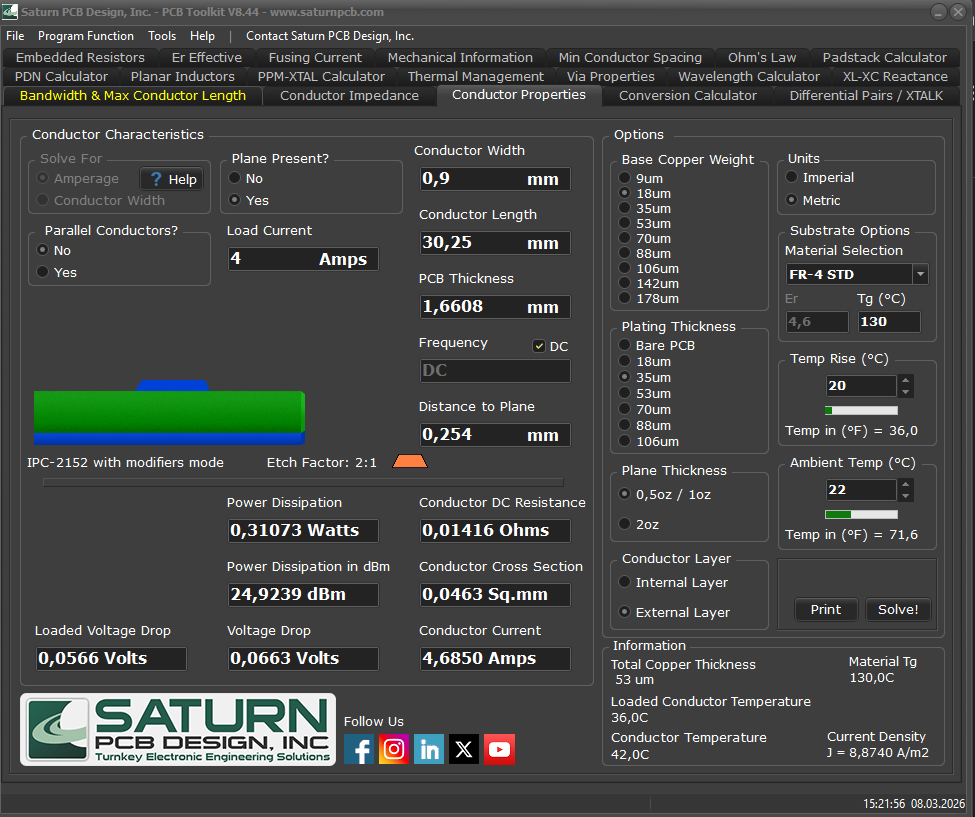
\includegraphics[width=0.5\linewidth]{Figures/inductor for upper pcb 4A.png}
    \caption[Conductor width ]{Conductor width for load of 4A for the upper PCB}
    \label{fig:inductor_width_upper_pcb}
\end{figure}

Additionally the via-points for the conductors moving through differnt planes, were also sized based on the Satrun PCB Design program, as shown in Figure~\ref{fig:via_points}. 

\begin{figure}[h]
    \centering
    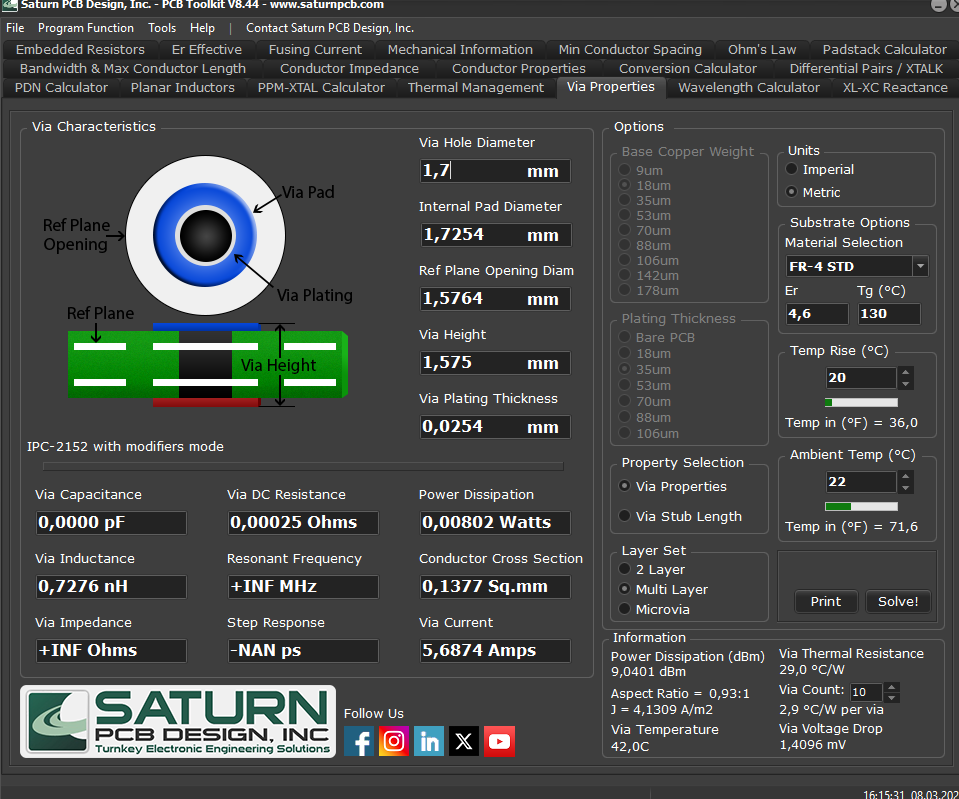
\includegraphics[width=0.5\linewidth]{Figures/via fot 5A.png}
    \caption[Via-point sizing]{Size of the via-point, that should hold for up to 5.5A}
    \label{fig:via_points}
\end{figure}

    \subsubsection{The upper PCB}
    The upper PCB is equiped in two voltage regulators of type \textbf{LM138}, where one provides the stepper-motors with 10V DC-supply, and the second provides 5V DC-supply to the Arduino nano and the Raspberry Pi. The output at the voltage regulators may be changed, by modifying the voltage ratio between the potentiometer and the restistor connected to the regulators output. The connection design was based on \cite{tiLM338}. The stepper-motors are controled by the \textbf{L6205}, which was connected according to \cite{stL6205}, where the control logic is provided by the connected Arduino nano. The compass module provided by MikroElektronika, which uses \textbf{HSCDTD008A}, was used to estimate the  relative postion of the tower. The connection diagram of the upper pcb can be seen in Figure~\ref{fig:connection_diagram_upper_pcb}, the 2D model in Figure~\ref{fig:2d_diagram_upper_pcb} and the 3D model in Figure~\ref{fig:3d_model_upper_pcb}.
    
    \begin{figure}[h]
        \centering
        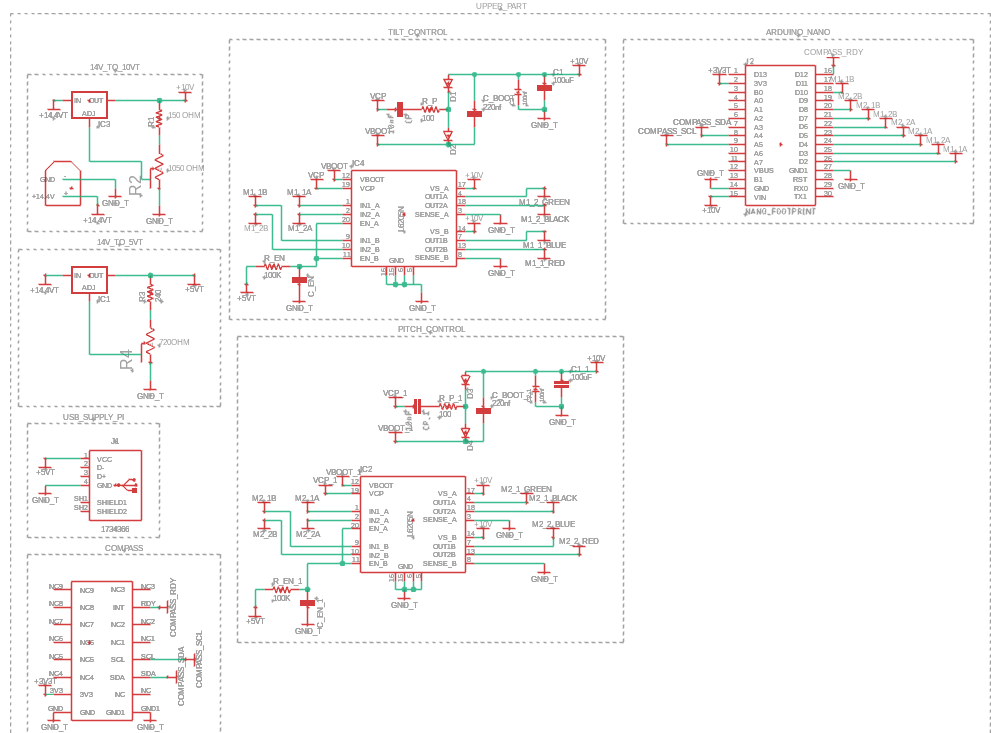
\includegraphics[width=0.75\linewidth]{Figures/upper_pcb_connection_diagram.png}
        \caption[  Connection diagram - upper PCB]{The connection diagram for the upper PCB.}
        \label{fig:connection_diagram_upper_pcb}
    \end{figure}
    \newpage
    \begin{figure}[h]
        \centering
        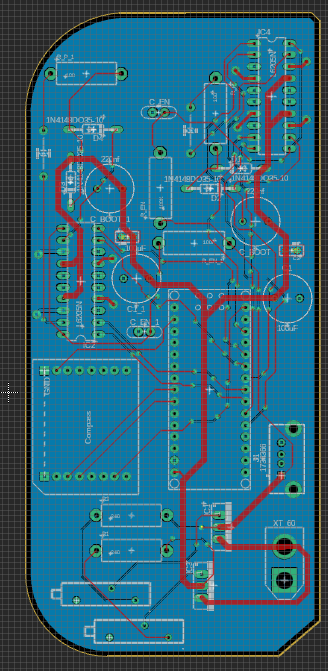
\includegraphics[width=0.25\linewidth]{upper_pcb_connections.png}
        \caption[  2D model - upper PCB]{The 2D model of the upper PCB.}
        \label{fig:2d_diagram_upper_pcb}
    \end{figure}
\newpage
    \begin{figure}[h]
        \centering
        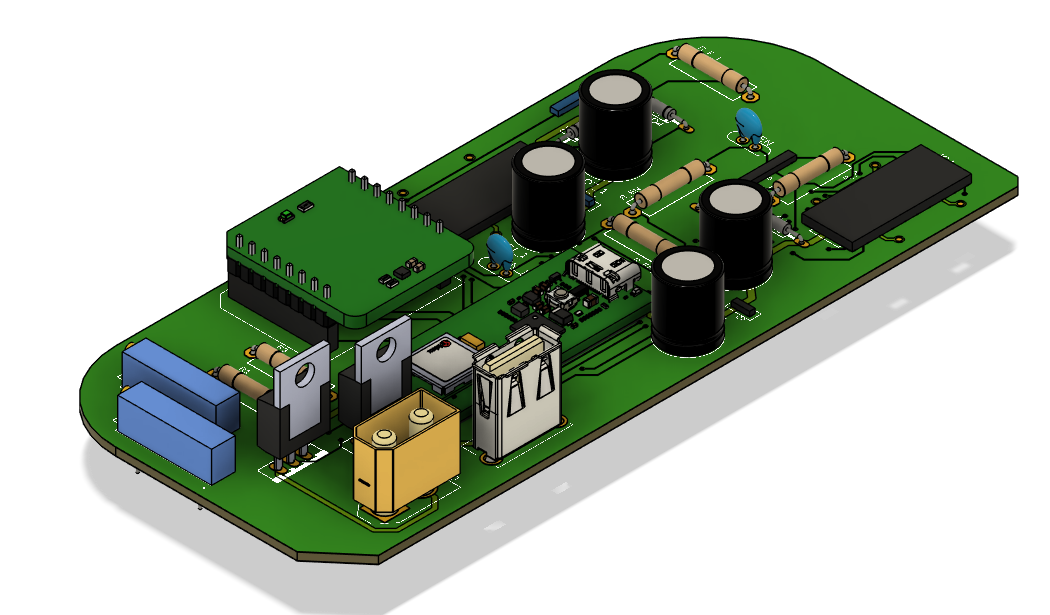
\includegraphics[width=1\linewidth]{Figures/upper_pcb_3d.png}
        \caption[  3D model - upper PCB]{The 3D model of the upper PCB}
        \label{fig:3d_model_upper_pcb}
    \end{figure}
    \newpage
    \subsubsection{Bottom PCB}
    The bottom PCB was meant to be used as the extantion board of the STM32 MCU, which was in high degree desgined based on the connection diagram of the CCA2M2 seen in \cite{x_nucleo_cca02m2_2019}. The bottom PCB just as the upper one, converts the voltage from the battery to 5V to supply the connected Raspberry Pi, and the STM32 MCU as can be seen in Figure~\ref{fig:connection_bottom_pcb}. The PCB allows for data signal from the micropohone pairs to be transferred on the same line, where one of the L/R pins of the microphones has to be put to ground, while the other to 3.3V. The Data from MCU in PCM format, is transferred to the Raspberry Pi/ PC through a microusb which is connected to an ESD unit composed of protection diodes. The 2D model of the bottom PCB can be seen in Figure~\ref{fig:2d_model_bottom_pcb}, and the 3D model in Figure~\ref{fig:3d_model_bottom_pcb},

    \begin{figure}[h]
        \centering
        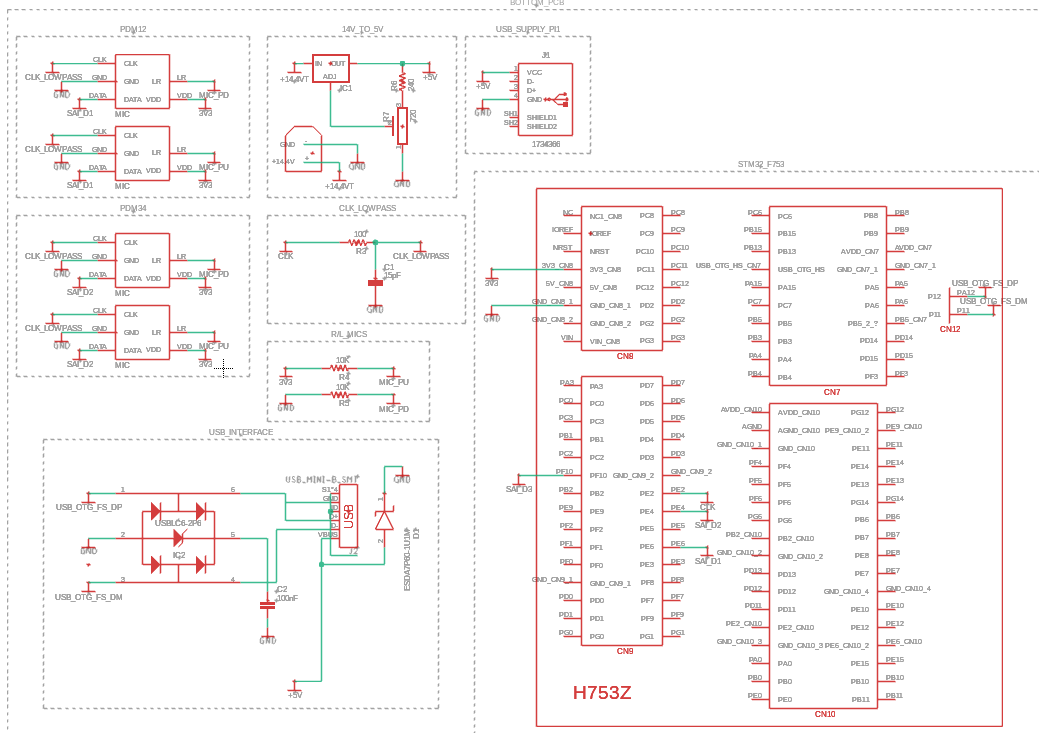
\includegraphics[width=0.75\linewidth]{Figures/connection diagram bottom pcb.png}
        \caption[  Connection diagram - bottom PCB]{The connection diagram for the bottom PCB.}
        \label{fig:connection_bottom_pcb}
    \end{figure}

    \begin{figure}[h]
        \centering
        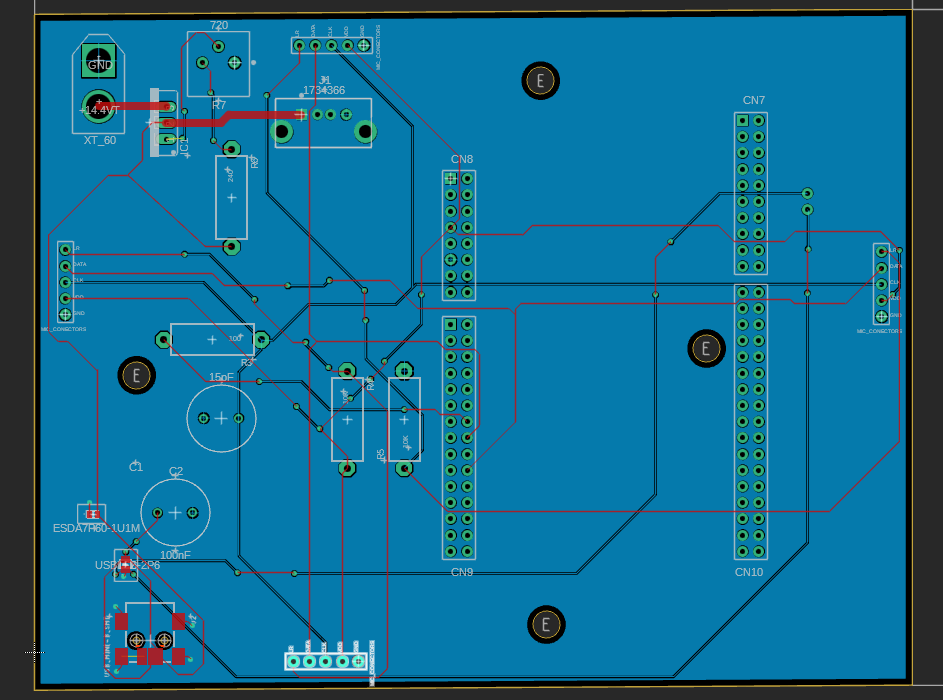
\includegraphics[width=0.5\linewidth]{Figures/2d_model_bottom_pcb.png}
        \caption[  2D model - bottom PCB]{The 2D model of the bottom PCB.}
        \label{fig:2d_model_bottom_pcb}
    \end{figure}

    \begin{figure}[h]
        \centering
        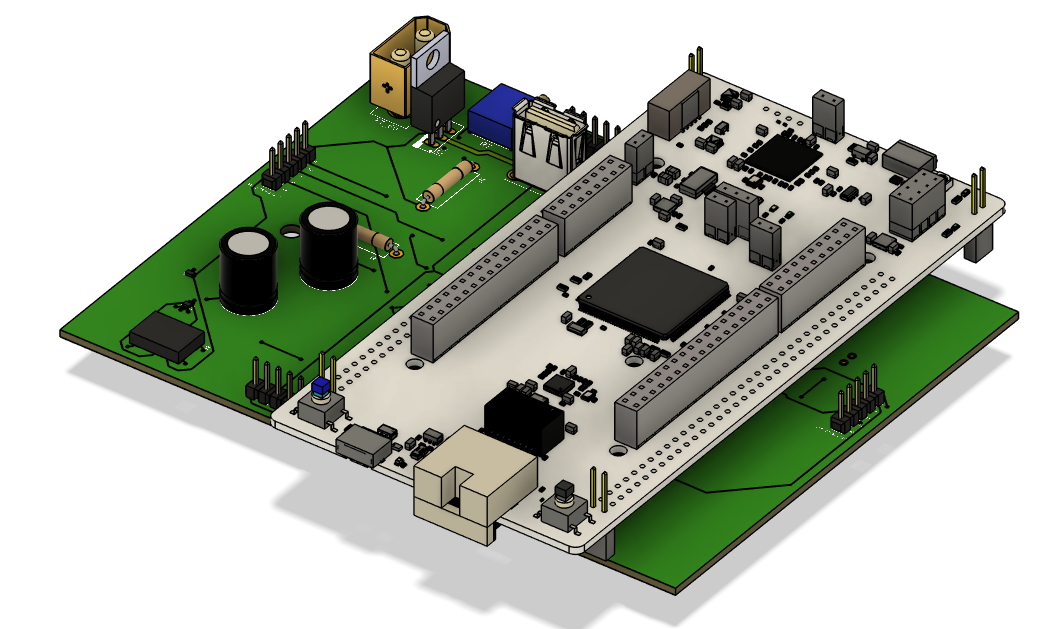
\includegraphics[width=0.85\linewidth]{Figures/3d_model_bottom_pcb.png}
        \caption[  3D model - bottom PCB]{The 3D model of the bottom PCB.}
        \label{fig:3d_model_bottom_pcb}
    \end{figure}
\newpage

\section{ML}
\subsection{YOLO implementation}

A YOLOV8n algorithm was trained on the drone dataset created by \cite{DroneDatasetFinal}. The drone dataset contains 51446 image training dataset of which there are 1 negative and 51445 positives. (\cite{DroneDatasetFinal}). The test dataset contained 5375 images of which there were 2750 negatives and 2625 positives (\cite{DroneDatasetFinal}). The classes were not balanced in the validation dataset in order to ensure that the model gets punished for false positives. mA NVIDIA RTX 4050 Laptop GPU was used during the training process with 32 GB DDR5 6400 MT/s of RAM. 

 \vspace{1em}
 
Following training, the model was exported from Ultralytics in ONNX format and converted to a Hailo Executable Format (HEF) file using the Hailo Dataflow Compiler (DFC) version 3.33.0, executed within the hailo8\_ai\_sw\_suite\_2025-10 Docker container running under WSL2. The conversion followed three sequential stages.
First, the ONNX model was parsed into a Hailo Archive (HAR) file using the hailo parser command. Because YOLOv8 uses a decoupled detection head, the six output nodes across the three detection scales were specified manually during parsing, following the node definitions provided in the Hailo Model Zoo yolov8n.yaml configuration file.
Second, the parsed HAR file was optimized using hailo optimize --hw-arch hailo8 --use-random-calib-set, which quantized the model weights from 32-bit floating point to 8-bit integer. The --use-random-calib-set flag was used in place of a representative calibration dataset, meaning quantization statistics were derived from randomly generated input data rather than real drone images.
Third, the optimized HAR was compiled to a HEF binary using hailo compiler --hw-arch hailo8. The compiler mapped the network across 8 on-chip clusters, with a total control utilization of 74.2\% and compute utilization of 43\%. Compilation completed in 9 seconds. The resulting drone\_detector.hef file was then deployed to the Raspberry Pi AI HAT+ for inference.

\subsection{YOLO testing}

In order to test the YOLO model on different drones in different settings 6 youtube videos containing drones were downloaded(tab: \ref{tab:test_videos}). The specific videos where chosen from a list of videos used by (\cite{DroneDatasetFinal}). The FLOUREON FPV racing drone video was shortened from 30 minutes to 15, due to the last 15 minutes being onboard drone footage, and therefore not useful for the qualitative test (\cite{floureon2017}). 
The YOLO model was also tested live in the lab on the flying drone, to verify that it works on the Raspberry PI. The confidence threshold used was 0.571, and it was found by anylising the F1 curve from the finished trained model. 

\begin{table}[H]
    \centering
    \caption{YouTube videos used for qualitative evaluation of the YOLOv8N drone detector.}
    \label{tab:test_videos}
    \begin{tabular}{llc}
        \toprule
        \textbf{Video} & \textbf{Drone type} & \textbf{Difficulty} \\
        \midrule
        Ryze Tello outdoor test \cite{tello2019}        & Consumer quadcopter & Easy   \\
        \$35 foldable drone review \cite{foldable2018}  & Toy quadcopter      & Easy   \\
        Karma vs Mavic vs Phantom 4 \cite{gopro2017}    & Multiple consumer   & Medium \\
        FLOUREON 250 FPV review \cite{floureon2017}     & FPV racing drone    & Medium \\
        Athletic power of quadcopters \cite{dandrea2016}& Indoor acrobatic    & Hard   \\
        IROS 2017 autonomous race \cite{iros2017}       & Indoor racing       & Hard   \\
        \bottomrule
    \end{tabular}
\end{table}


\subsection{Sound classification}
The project employs two distinct machine‑learning algorithms for the classification of detected sounds. Each incoming sound is automatically labelled either as “Drone” or “Not-a-drone”. Both models are implemented in Python, using Librosa for handling of Mel‑frequency cepstral coefficient (MFCC) objects. The models were trained on a combination of a public dataset(\cite{AudioDatasett}) and data collected with the microphone array. 

1. Convolutional Neural Network (CNN).
This model is a Convolutional Neural Network built with TensorFlow(version-2.21.0). The network operates on MFCC-spectrograms and learns hierarchical feature representations that discriminate drone from non‑drone sounds.

2. Accumulative‑Feature Decision‑Tree Classifier.
The second model is a decision‑tree classifier that utilizes accumulative statistics of the mel‑spectrogram and the MFCCs—specifically the mean and standard deviation across time frames. It is implemented with scikit‑learn (a.k.a. sklearn)(version-1.8.0).


\section{Communication}

\subsection{RPI to Arduino}
A MQTT publisher subsriber scheme was used for the communication between the upper RPI and the Arduino using the mosquito library with the RPI acting as a host. There are two topics on the broker, one for the pixel coordinates, and the other for the compass readings. 


\subsection{RPI camera pipeline}

OpenCV was used to capture the video footage from the RPI camera. The frames were then accessed by two separate threads. The first thread is the YOLO thread which takes the frame and converts it to the correct format for the YOLO algorithm. The YOLO algorithm is then performed and the pixel coordinates of the detected drone is then publish on the coordinates topic. After the YOLO thread has accessed the frame, the camera sender thread accesses it and encodes it using the H.264 format. The frame is then sent via a UDP socket created by the boost asio library to the webserver which displays the camera feed with the GUI. 

\begin{figure}[H]
    \centering
    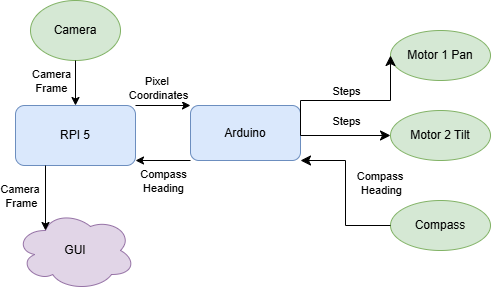
\includegraphics[width=0.5\linewidth]{Figures/Andreas/Flowcharts/Camera_flowchart.png}
    \caption[Communication flowchart]{Flowchart showing the communication bewteen devices}
    \label{fig:placeholder}
\end{figure}

\begin{figure}[H]
    \centering
    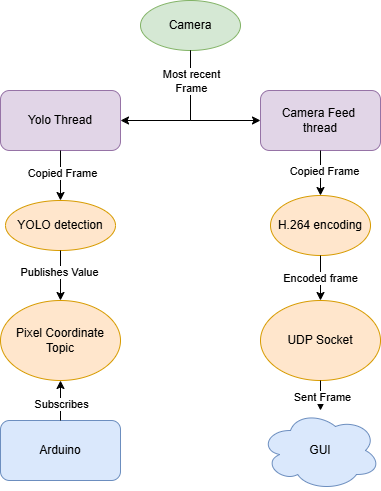
\includegraphics[width=0.5\linewidth]{Figures/Andreas/Flowcharts/Camera_pipeline.png}
    \caption[Camera pipeline flowchart]{Flowchart showing the different threads in the camera pipeline}
    \label{fig:placeholder}
\end{figure}

\section{GUI}
The graphical user interface (GUI) was deliberately engineered to be minimalist and support rapid prototyping, thereby accommodating the evolving requirements that arise throughout the development lifecycle.The design process initiated with a preliminary wireframe that outlined the core components of the GUI page; this sketch subsequently evolved into the wireframe presented in Figure-Add.The GUI was intended to run on a Raspberry-Pi functioning as a web server, which interfaces with the microphone array.

The server was implemented in plain JavaScript to satisfy the storage constraints of the Raspberry-Pi. Docker was employed to construct a reproducible image of the server, enabling rapid testing and updates on an external microcomputer (Raspberry-Pi). The server operates as an HTTPS‑secured service, granting access to the device’s GPS location.

\section{Tests performed}
\subsection{Sound signal acquisition}
The acoustic data signal from the microphones was received using two distinct peripherals on three different STM32 based controllers. The first peripheral used is SAI, and was tested on the  STM32F446 and STM32H753 controllers. The second peripheral tested was the DFSDM which was applied on the STM32F413 MCU. 

\subsubsection{SAI acquisition tests}
The sound acquisition test was conducted by placing the microphone platform seen in Figure~\ref{fig:first_mic_platform}, in the middle of an empty classroom. The test was conducted by one student, whom spoke to the microphones in the distance of around 2 meters. The main objective of the test was to evaluate wether the acquired microhpone signals could be used by the DOA algorithm, which at that stage of the project, was expected to estimate the direction of the strongest sound source.\\

\begin{figure}[h]
        \centering
        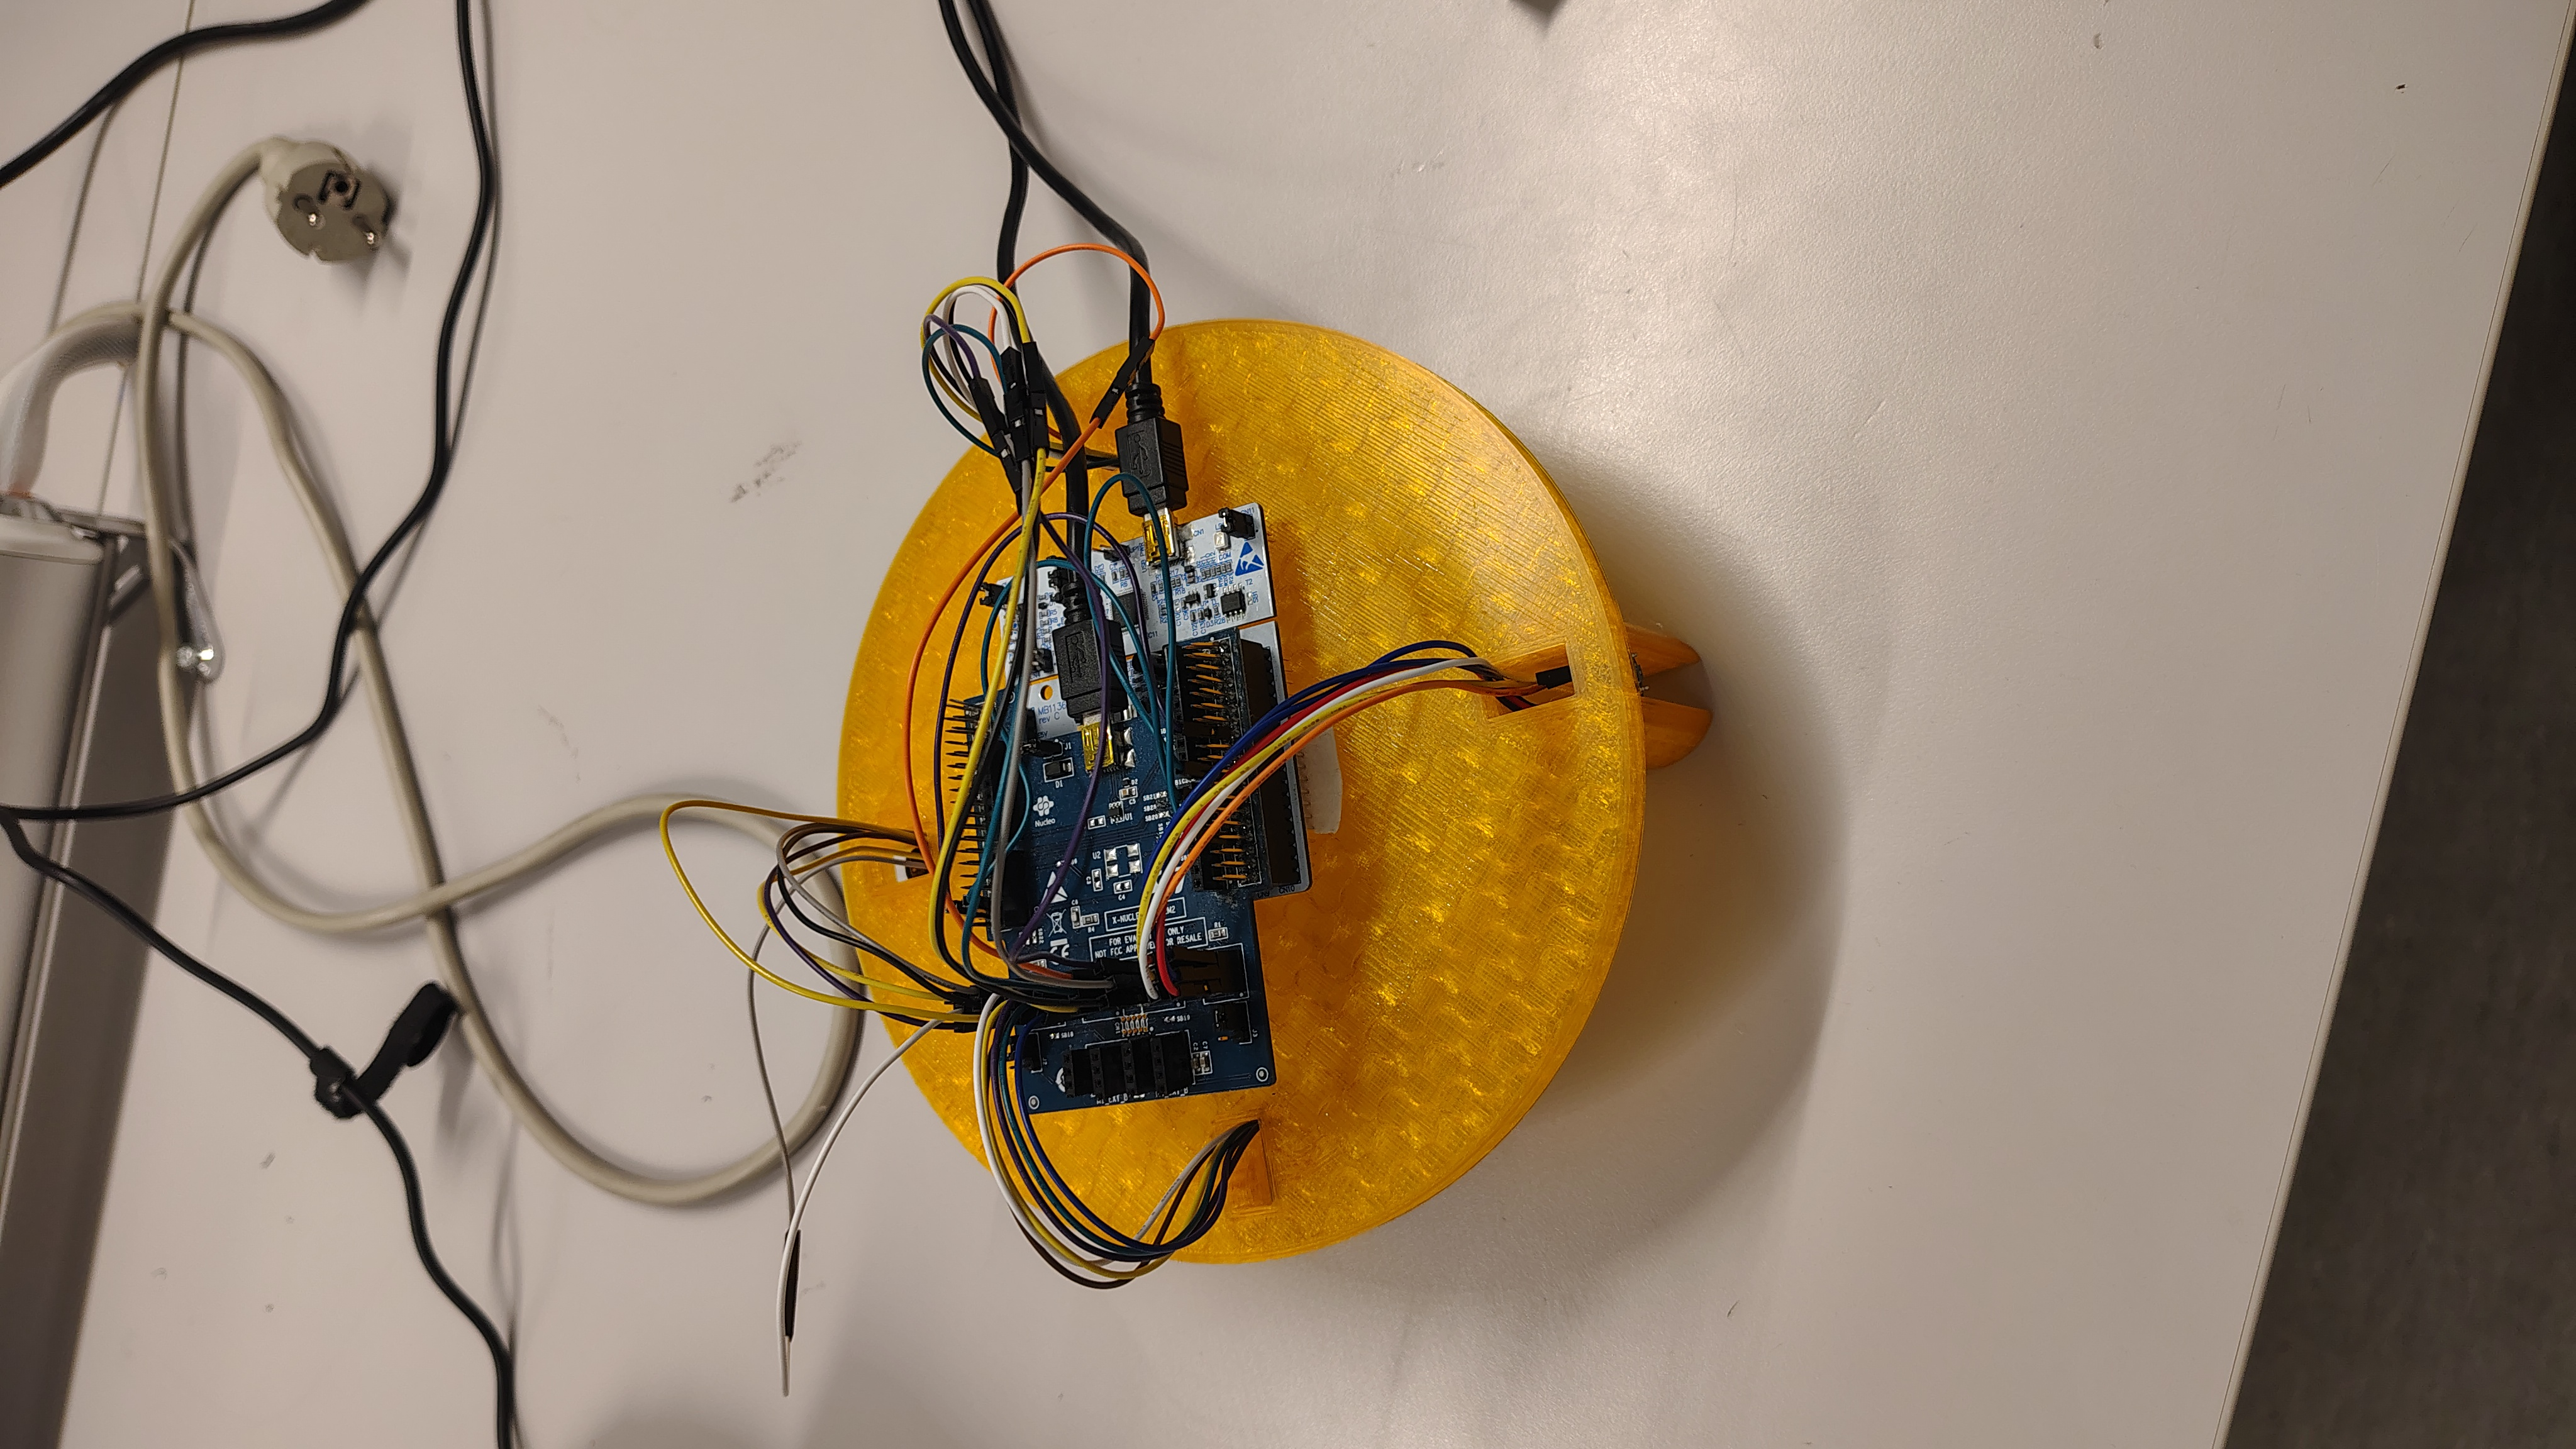
\includegraphics[width=0.5\linewidth]{Figures/IMG_20260220_212107140_HDR.jpg}
        \caption[The microphone first platfrom]{The first microphone platform design used for testing of the sound acquisition pipeline}
        \label{fig:first_mic_platform}
    \end{figure}
\newpage
\subsubsection{DFSDM acquisition tests}
After several trials with the SAI peripheral, the acquisition method was changed from SAI to DFSDM. This also required changing the MCU to the STM32F413, which supported the DFSDM peripheral used in the final implementation. A more detailed explenation of this peripheral change is given in Section~\ref{sec:stm32_models_reasoning}.\\

The DFSDM acquisition test was conducted in the same way as the previous SAI tests, where one student spoke or clapped towards the microphone platform from a distance of approximatley 2 to 7 meters.

\subsection{DOA estimation tests}
Testing of the DOA estimation module was conducted in three different stages
after the DFSDM peripheral was implemented in the system. The purpose of the first stage was to verify whether the system could estimate the direction of the dominant acoustic source under simple test conditions, while the two other stages mainly focused on DOA estimation of the actual drone sounds.

\subsubsection{Stage 1: Human-generated sounds}
The first stage used the human speech and clapping sounds, as the test signals.
These sounds were produced at distances of up to 2 meters from the microphone platform, both in an empty classrom and in a classroom occupied by other students. The test signals were used because they were easy to produce repeatedly ,during testing and made it possible to quickly evaluate the behaviour of the DOA algorithm, before testing it with the drone sounds.

\subsubsection{Stage 2: Recorded drone and drone-like sounds}
The second stage of the testing process used the sound made by a DC-motor supplied by 6V and drawing around 200 mA, and a recorded drone sound taken from Youtube, that can be accessed in: \href{https://www.youtube.com/watch?v=gA7-gb7l3Fc}{The drone sound video from youtube}. The purpuse of this testing stage, was to verify if the system is able to detect the sound made by the drone, or drone like sounds.\\

The test involving the drone video, was conducted by placing the mobilephone in the distance of around 7 meters away from the station, and at an angle of approx. -90 degrees relative to the station. The volume on the phone was turned to the maximum, while playing the drone video for the first test, and was later reduced to approx.50\% and 5\%. \\

Additionally the root-mean-square or simply (RMS) value was used as a relative measure of signal magnitude, as it seamed to be a more suitable in  describing the varying signal than a simple average, based on \cite{openlearn_rms}. The code used to generate the RMS can be seen in Code~\ref{lst:rms}, and is based on \cite{oxford_rms}.\\

\newpage

\begin{lstlisting}[style=pythonstyle, caption={logic for calculating the RMS per channel}, label={lst:rms}]
rms_per_channel = np.sqrt(np.mean(df**2))
\end{lstlisting}

%The energy level in db, was found by using Equation~\ref{eq:log_phone_volume}.

%\begin{equation}
%    \label{eq:log_phone_volume}
%    Relative \space level= 20\log_{10}(\frac{level_{test}}{level_{100}})
%\end{equation}

\subsubsection{Stage 3: Live drone test}
The third and the last stage of the DOA estimation testing, was conducted by using the drone present at the visualization lab. The first series of tests did not involve the use of the ML or the camera, and the setup was as seen in Figure~\ref{fig:doa_3_stage_no_camera}. Where the bottom part of the tower, with the microphones mounted on it, was placed in the middle of the laboratory. \\

The system was first tested without the drone present, in order to observe the background noise level in the laboratory, which would be later used as a baseline, to compare the frequency content of the room noise, with the frequency content produced when the drone was flying.


\begin{figure}[h]
    \centering
    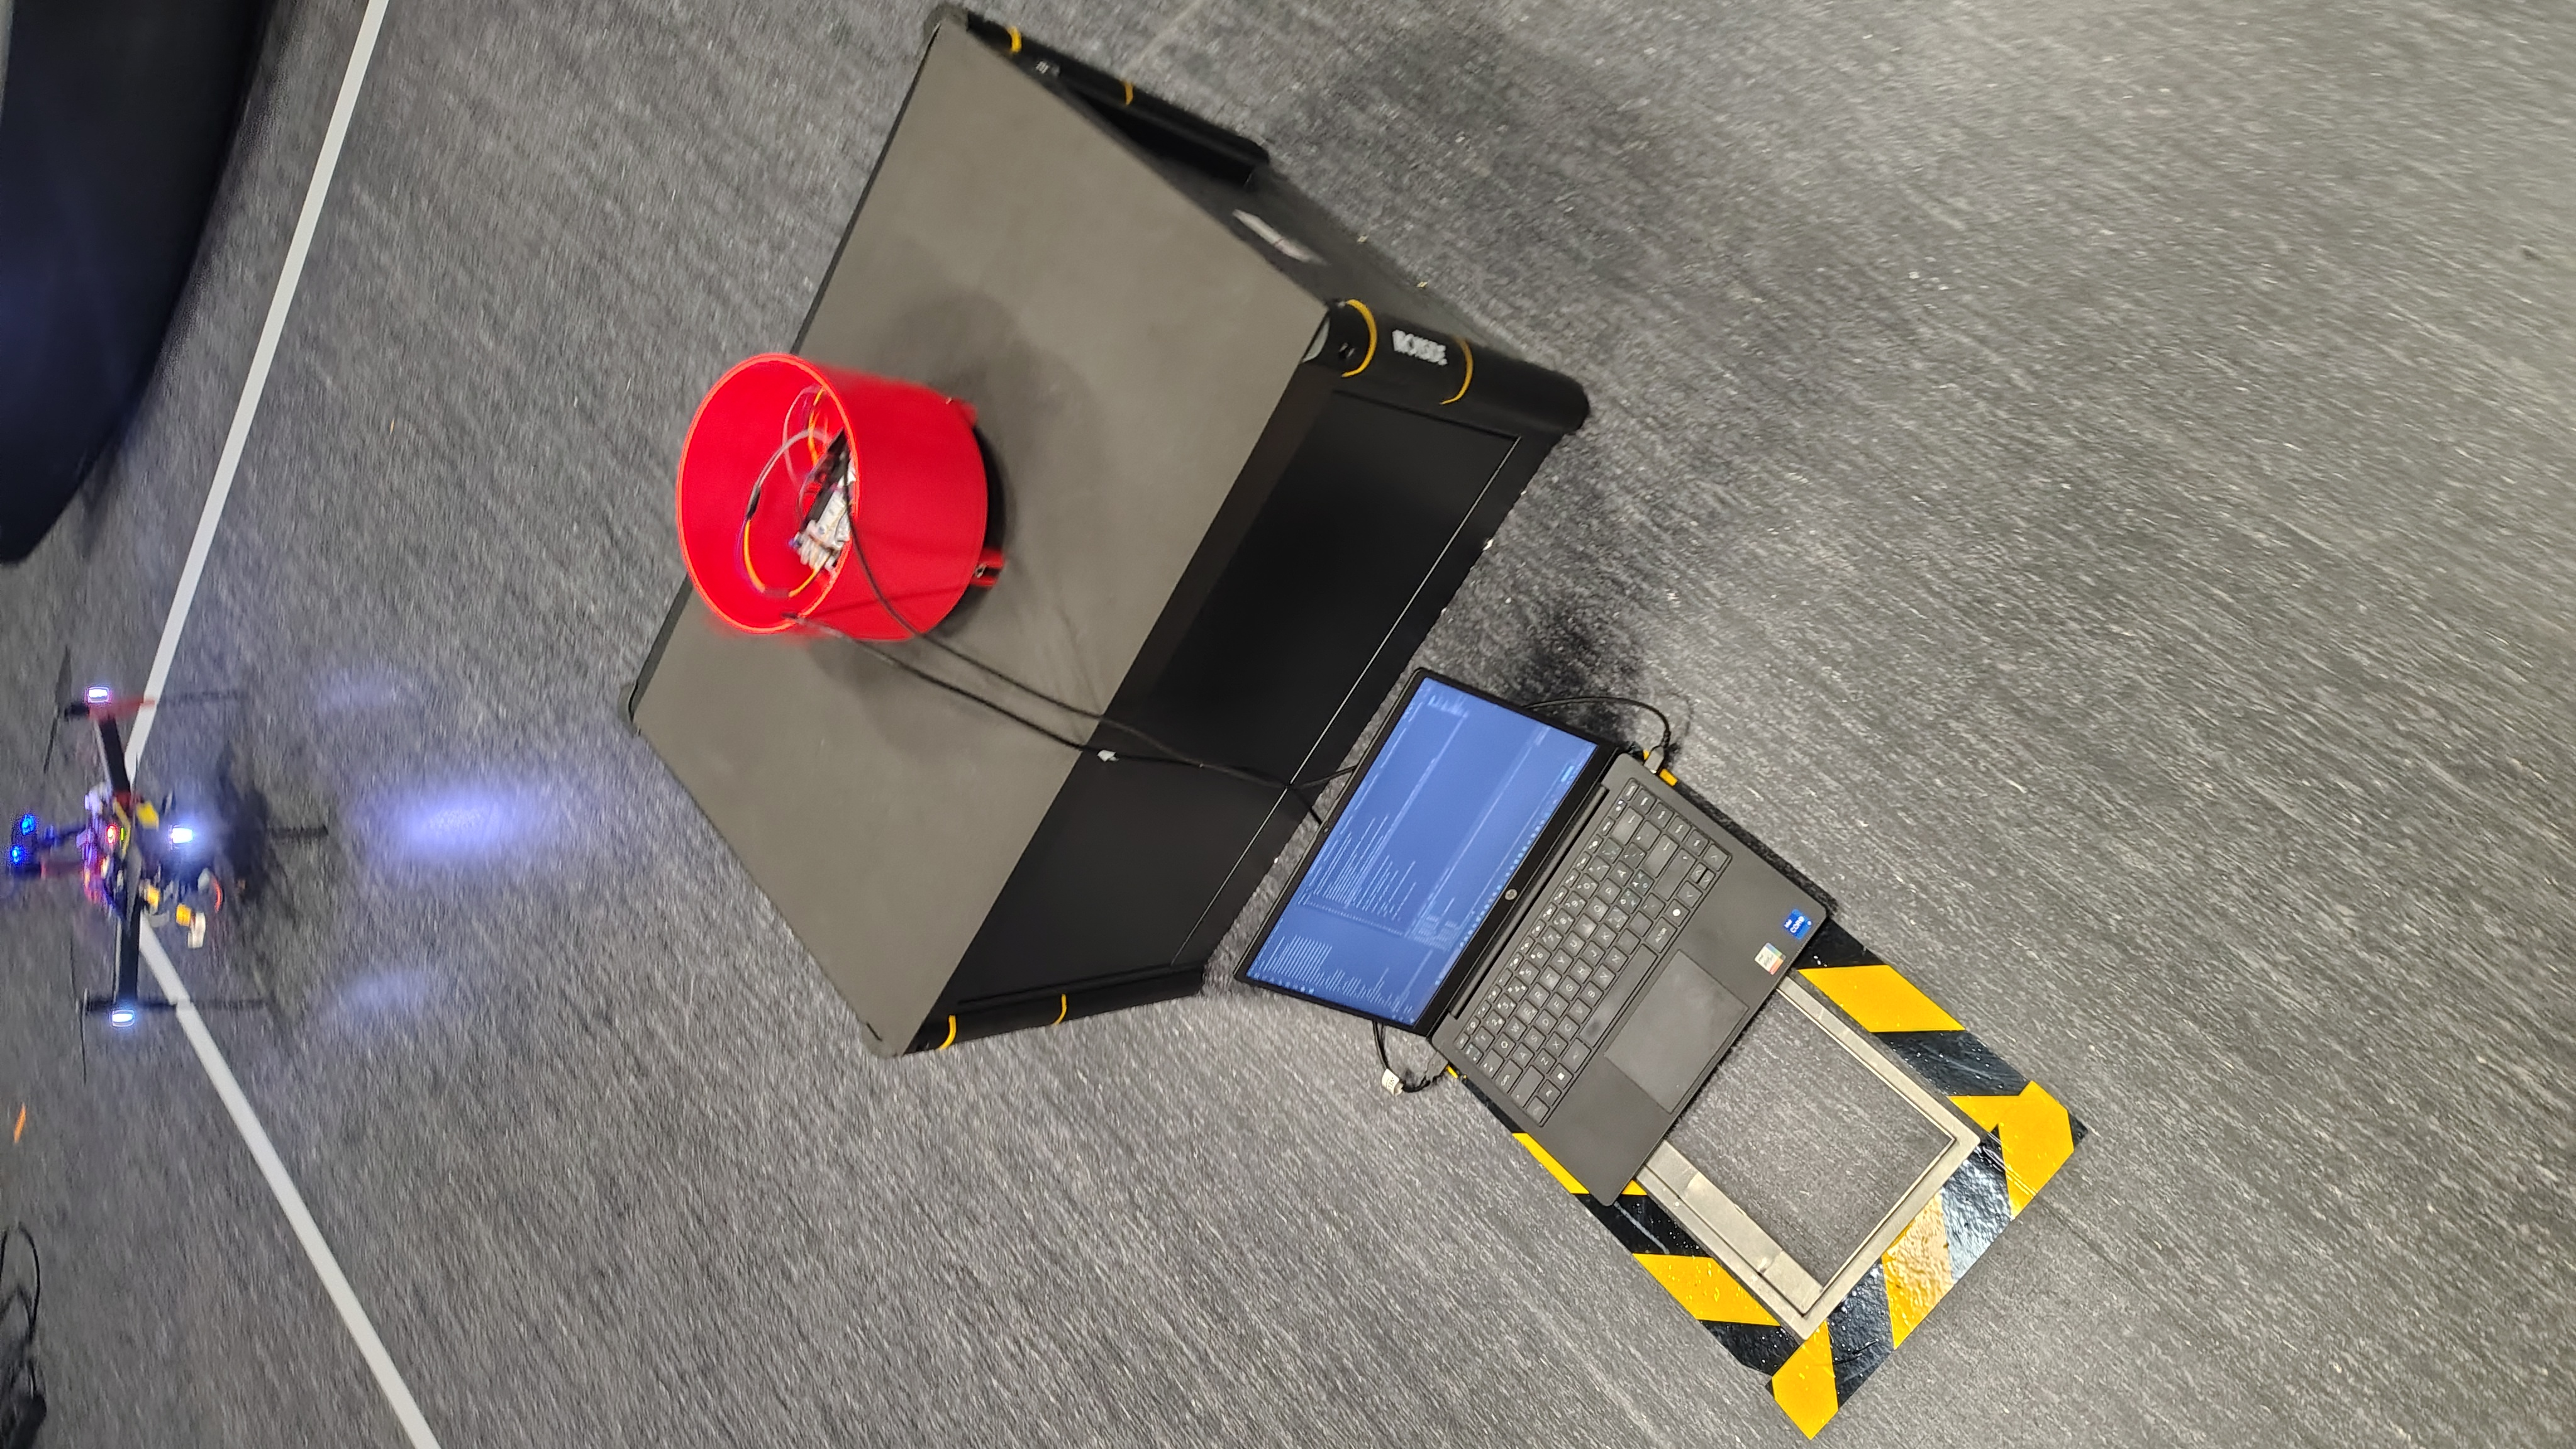
\includegraphics[width=0.5\linewidth, angle=-90]{Figures/1000001927.jpg}
    \caption{The first test in the third stage of the DOA estimation testing}
    \label{fig:doa_3_stage_no_camera}
\end{figure}

The next test involved the use of the live-drone which was circulating around the tower, while the system was processing the acquired sound to estimate the DOA.\\
\newpage
The final test was conducted after the ML-algorithm togheter with the camera was implemented in the system, where the test enviroment would be the same as for the previous tests as seen in Figure~\ref{fig:doa_3_stage_setup}.\\ 

\begin{figure}[h]
    \centering
    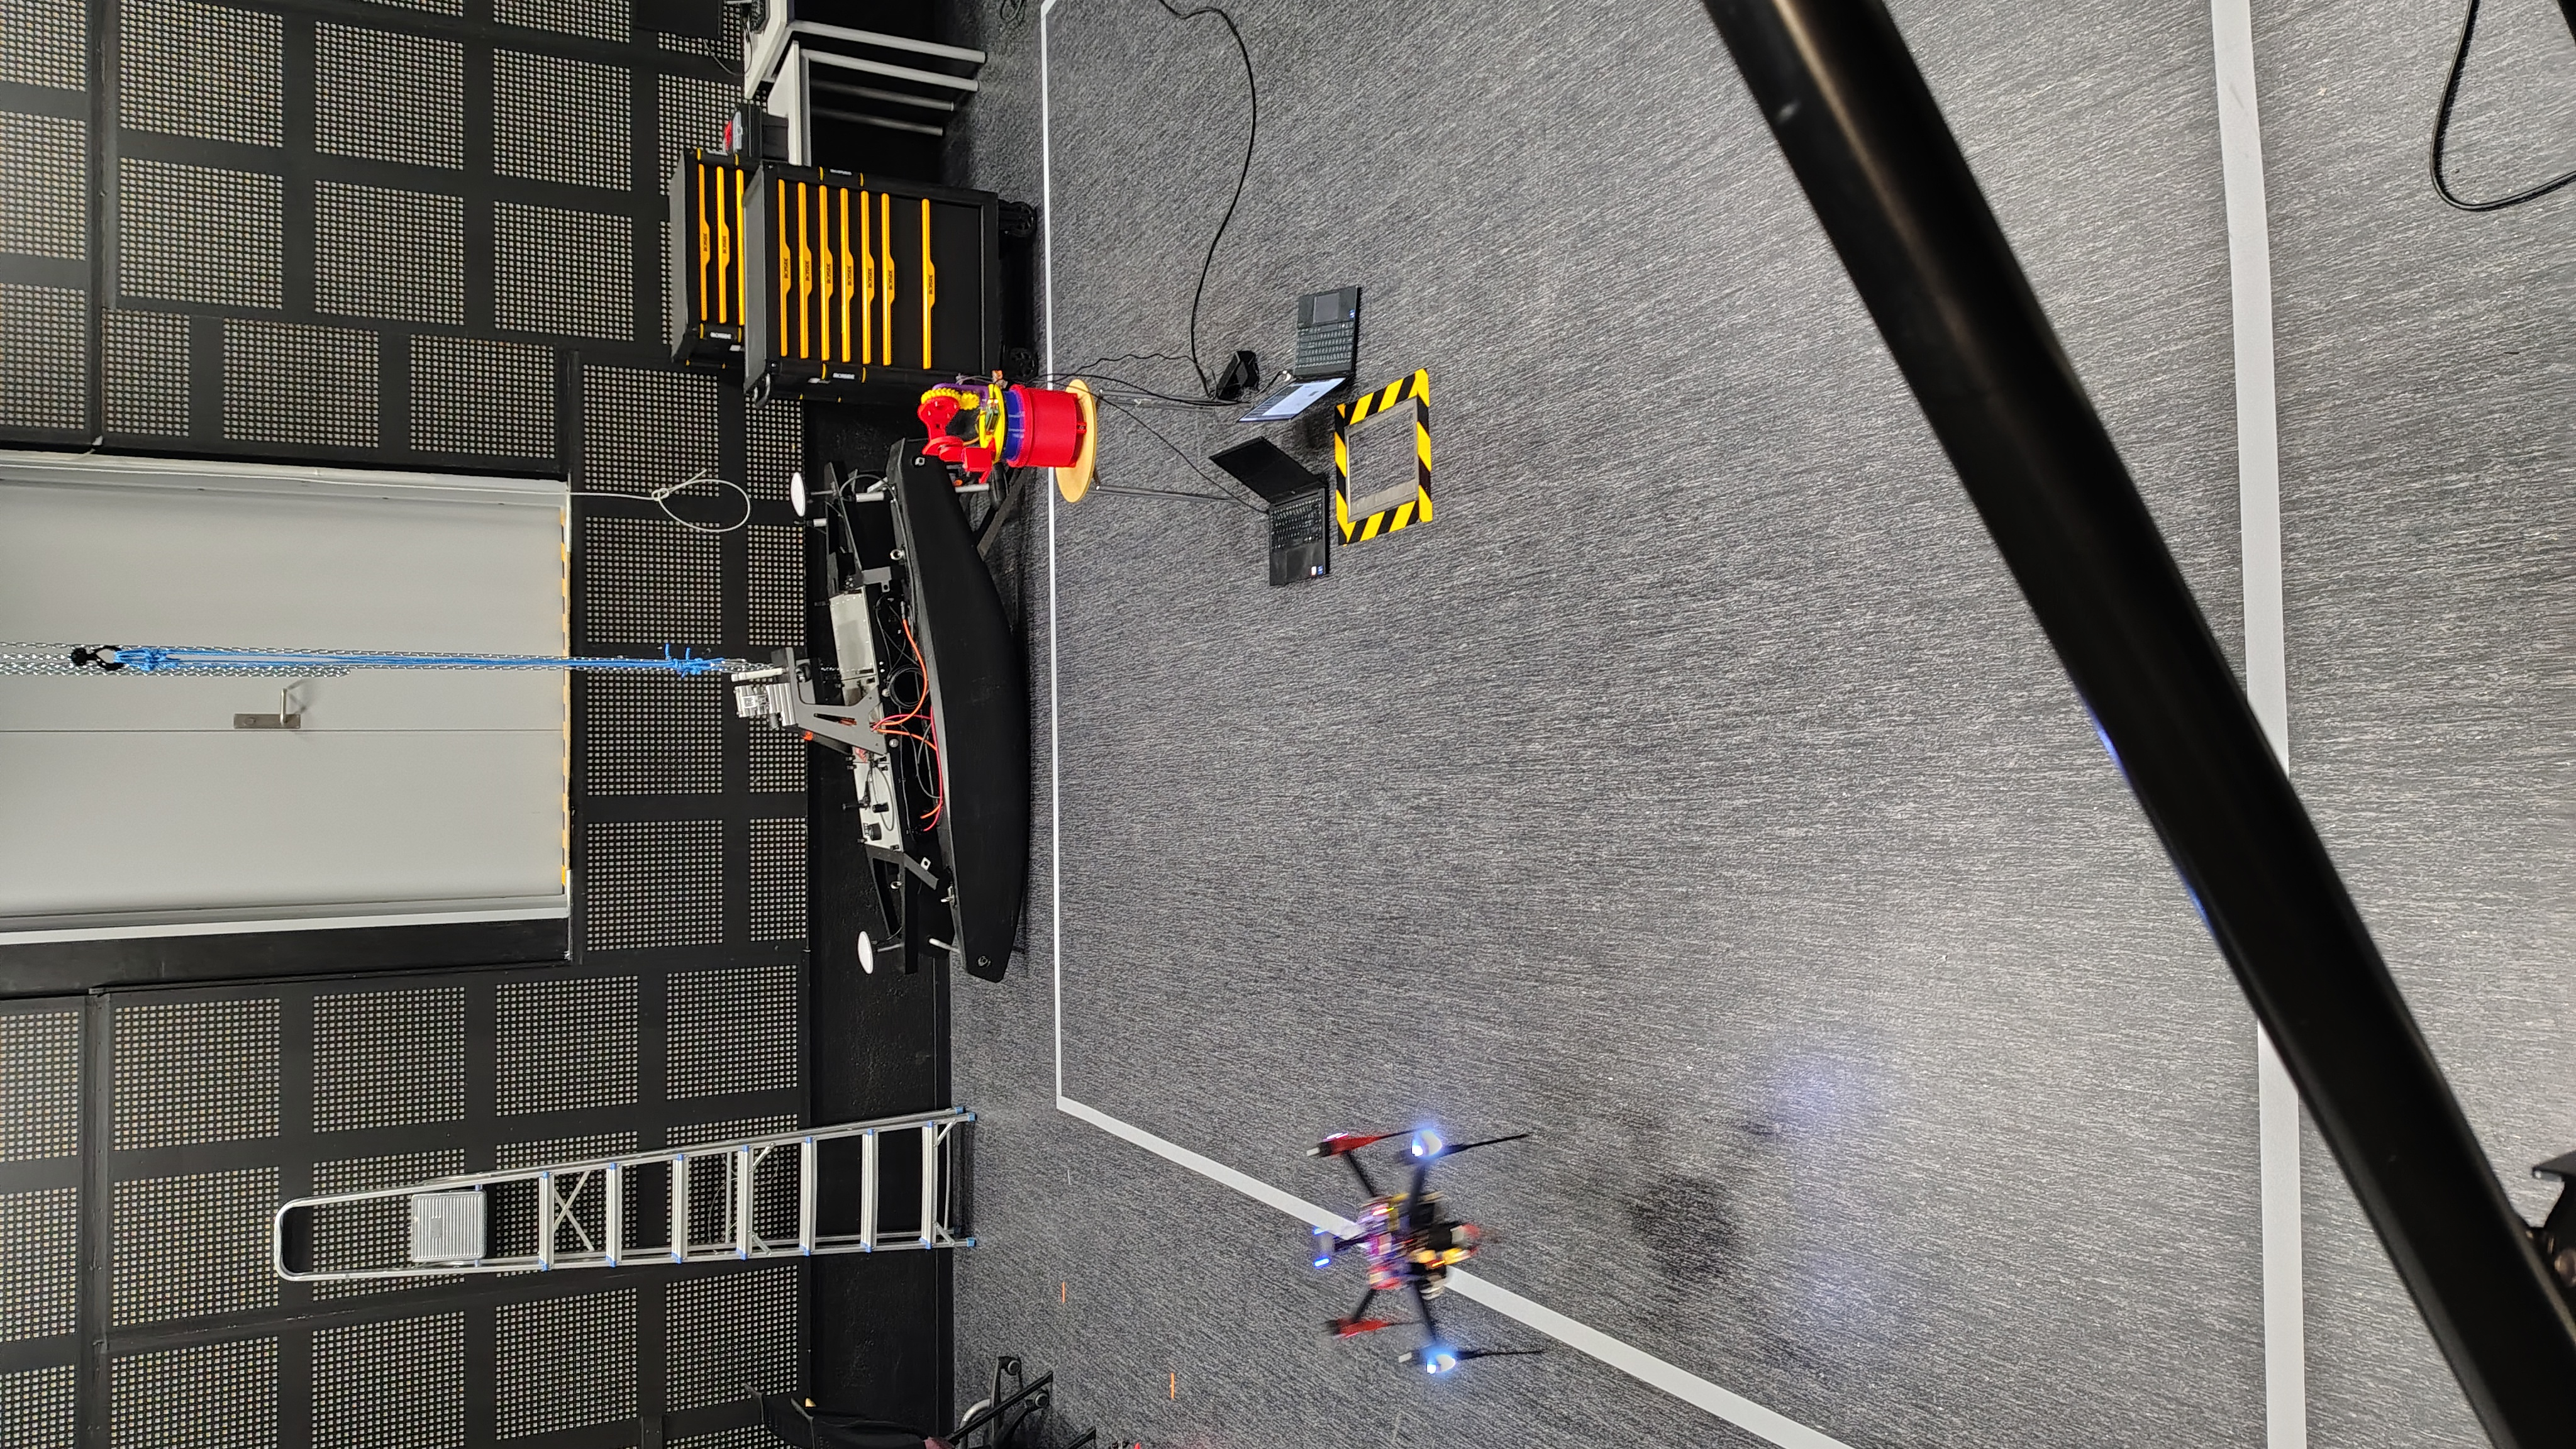
\includegraphics[width=0.5\linewidth, angle=-90]{Figures/IMG_20260514_115338104_HDR.jpg}
    \caption{Setup for the third DOA testing stage}
    \label{fig:doa_3_stage_setup}
\end{figure}
\newpage
The ML was tested by letting the system record the sound without the drone present. The system was expected to return the "Not a drone" flag, which would not allow for the DOA estimation to be conducted, and later the drone would be flown, so that the ML could return the "drone" falg and allow for DOA estimation.\\

After the ML algorithm was verified, the final test was conducted, where the drone was flawn around the tower, in varying distance but not outside the safety area designated in the laboratory ,due to the safety conserns. The system was expected to accurately produce a DOA estimation as it was proven possible in the previous tests. Since the drone was to be in constant circulation around the tower, it was expected that the DOA estiamtion will lag behind the drone with a lag of atleast 1 second, due to the duration of the recorded sound, and some additional overhead caused by the other modules in the system.\\  

\subsection{Hardware test}

In order to test the hardware requirements of running a YOLO model on a raspberry pi 5 a stress test was performed while logging the CPU usage, temperature as well as the RAM usage of the system. Interference time was also measured while the YOLO model was run by the system. The test was performed while utilising the HAILO chip, as well as running the model on the CPU only. 

\subsection{Project Management}
The Development team employed the Scrum framework to organise the work. The project was split into bi-weekly sprints. At the end of each sprint the team performed a sprint-review, during which the team went over what was accomplished and what needed to be done by the next sprint.

The product owner, Erlend-Magnus-Lervik-Coates (NTNU-Dronelabben), participated in all review meatings and some planning meatings. The backlog was managed with Github Issues, which served as the source of user stories, bug reports and task assignments.





%\section{Signal Processing Implementation}
% Maybe split into GCC and MFCC?
% ADD the influence that SNR has on confidence of a segment in gcc!
% “A confidence measure based on the ratio between the correlation peak and the average energy in the segment is used to discard unreliable frames. This can be interpreted as a local SNR estimate.” ? 
%    \subsection{Frame length}
%    \subsection{Windowing}
%    \subsection{FFT size}
%    \subsection{PHAT implementation}
%    \subsection{Sub-sample interpolation}
%    \subsection{Confidence filtering}

%\section{Feature Extraction}
%    \subsection{MFCC}
%    \subsection{ML}